\documentclass[ngerman,openany, oneside]{Script}
\usepackage{amsmath}


% Aufgabentext ein-/ausschalten
\newboolean{aufgabentext}
\setboolean{aufgabentext}{true}
\newcommand{\aufgabentext}[1]{\ifthenelse{\boolean{aufgabentext}}{#1}{}}

% Wenn aufgabentext auch true ist, dann wird der Lösungstext etwas abgesetzt und kursiv geschrieben
\newboolean{mitloesung}
\setboolean{mitloesung}{false}
\newcommand{\loesung}[1]{\ifthenelse{\boolean{mitloesung}}{\ifthenelse{\boolean{aufgabentext}}{{~\\\itshape{#1}}}{#1}}{}}

% Für die Strukturierung
\newcommand{\Thema}[1]{\chapter{#1}}
\newcommand{\Thementeil}[1]{\section{#1}}
\newcommand{\Aufgabe}[1]{\subsection{#1}}
\newcommand{\Unteraufgabe}[1]{\subsubsection{#1}}
\newcommand{\Lernziele}[1]{\subsection*{Lernziele}{#1}}
\graphicspath{{./Bilder/}}

\newcommand{\mucho}[8]{
	\aufgabentext{
	\begin{enumerate}
	\item[#1] \emph{\textbf{#2}} #3
		\begin{enumerate}
		\itemsep1pt\parskip0pt\parsep0pt
		\item[A] #4
		\item[B] #5
		\item[C] #6
		\item[D] #7
		\loesung{Lösung: #8}
		\end{enumerate}
	\end{enumerate}
	}}

\begin{document}

\titelseite[Christian Stoll\\ Sebastian Lange]{Das Praxisskript }%
	{für den Amateurfunkkurs Klasse A}%
	{SoSe 2016}%

\newpage
\thispagestyle{empty}

\begin{tabular}{p{13cm} p{1cm}}
\textbf{Impressum} &\\
&\\
Titel: Praxisskript der Projektwerkstatt DK0TU&\\
Autor: Christian Stoll&\\
1. Auflage Juni 2016 &\\
&\\
Erschienen im :&\\
Fachgebiet Hochfrequenztechnik &\\
Institut für Hochfrequenz- und Halbleiter-Systemtechnologien&\\
Fakultät IV - Elektrotechnik und Informatik &\\
Sekr. HFT 4 &\\
Raum HFT 307 &\\
Einsteinufer 25 &\\
D-10587 Berlin &\\
&\\
Leitung: Prof. Dr. Klaus Petermann &\\
&\\
&\\
%Abbildung:&\\
&\\
Aktuelle Informationen der Projektwerkstatt finden Sie unter:  &\\
\url{http://www.dk0tu.de} &\\
&\\
Die vorliegende Fassung des Praxisskripts wurde sorgfältigst auf Fehler hin überprüft. Um das Praxisskript dennoch laufend verbessern zu können, würden wir uns über Hinweise auf etwaig vorhandene Fehler sowie Verbesserungsvorschläge sehr freuen. Wenden Sie sich dazu bitte an die Tutor\_innen und wissenschaftlichen Mitarbeiter\_innen der Projektwerkstatt. &\\
\end{tabular}




\newpage
%%Inhaltsverzeichnis
\tableofcontents
\newpage

\newpage

\chapter{Der Widerstand}
\begin{wrapfigure}[0]{r}[-1cm]{3cm}
 \vspace{-5cm}
 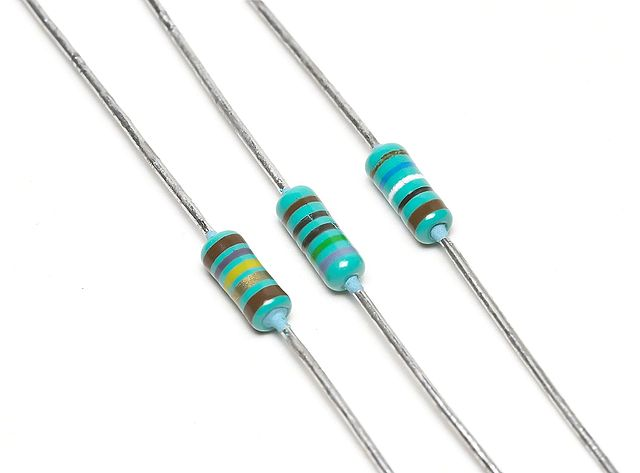
\includegraphics[scale=0.9]{Widerstand/Bilder/Resistors.jpg}
 \vspace{-5cm}
\end{wrapfigure}

\section*{Theorie- und Prüfungsfragen} 

\aufgabentext{
	\begin{enumerate}
	\item[1] \emph{\textbf{TB102}} Welchen Widerstand hat eine Kupferdrahtwicklung, wenn der verwendete Draht eine Länge von 1,8 m und einen Durchmesser von 0,2 mm hat
		\begin{enumerate}
		\itemsep1pt\parskip0pt\parsep0pt
		\item[A] 0,05 $\Omega$
		\item[B] 1 $\Omega$
		\item[C] 5,6 $\Omega$
		\item[D] 56 $\Omega$
		\loesung{Lösung: B}
		\end{enumerate}
	\end{enumerate}
}

\aufgabentext{
	\begin{enumerate}
	\item[2] \emph{\textbf{TC315}} Was verstehen Sie unter dem technischen Ausdruck Skin-Effekt?
		\begin{enumerate}
		\itemsep1pt\parskip0pt\parsep0pt
		\item[A] Als Skin-Effekt bezeichnet man die Erscheinung, dass sich mit steigender Frequenz der Elektronenstrom mehr und mehr zu den Kanten eines Kondensators hin verlagert. Dadurch erhöht sich mit steigender Frequenz die Kapazität.
		\item[B] Als Skin-Effekt bezeichnet man die Erscheinung, dass sich mit steigender Frequenz der Elektronenstrom mehr und mehr zur Oberfläche eines Leiters hin verlagert. Dadurch erhöht sich mit steigender Frequenz der Leiterwiderstand.
		\item[C] Als Skin-Effekt bezeichnet man die Erscheinung, dass sich mit steigender Frequenz die Induktivität und die Kapazität eines Leiters erhöht. Dadurch erhöht sich mit steigendem Leiterwiderstand die Resonanzfrequenz.
		\item[D] Als Skin-Effekt bezeichnet man die Erscheinung, dass sich mit steigender Frequenz der Elektronenstrom mehr und mehr zur Leitermitte hin verlagert. Dadurch erhöht sich der Leiterwiderstand bei hohem Wechselstromanteil.
		\loesung{Lösung: B}
		\end{enumerate}
	\end{enumerate}
}

\mucho{3}{TC102}
{Metallschichtwiderstände}
{haben geringe Fertigungstoleranzen und Temperaturabhängigkeit und sind besonders als Präzisionswiderstände geeignet.}
{sind induktionsarm und eignen sich besonders für den Einsatz bei sehr hohen Frequenzen.}
{sind besonders als Hochlastwiderstände bei niedrigen Frequenzen geeignet.}
{haben einen extrem stark negativen Temperaturkoeffizienten und sind besonders als NTC-Widerstände (Heißleiter) geeignet.}
{A}

\mucho{4}{TC103}
{Metalloxidwiderstände}%Frage
{haben geringe Toleranzen und Widerstandsänderungen und sind besonders als Präzisionswiderstände in der Messtechnik geeignet.}%A
{sind besonders als Hochlastwiderstände bei niedrigen Frequenzen geeignet.}%B
{sind induktionsarm und eignen sich besonders für den Einsatz bei sehr hohen Frequenzen.}%C
{haben einen extrem stark negativen Temperaturkoeffizienten und sind besonders als NTC-Widerstände (Heißleiter) geeignet.}%D
{C}%Lösung

\mucho{5}{TC104}
{Drahtwiderstände}%Frage
{Drahtwiderstände werden hauptsächlich in Form von SMD-Widerständen hergestellt.}%A
{sind induktionsarm und eignen sich besonders für den Einsatz bei sehr hohen Frequenzen.}%B
{haben einen extrem stark negativen Temperaturkoeffizienten und sind besonders als NTC-Widerstände (Heißleiter) geeignet.}%C
{sind besonders als Hochlastwiderstände bei niedrigen Frequenzen geeignet.}%D
{D}%Lösung

\mucho{6}{TB202}
{Die Leerlaufspannung  einer Gleichspannungsquelle beträgt 13,5 V. Wenn die Spannungsquelle einen Strom von 0,9 A abgibt, sinkt die Klemmenspannung auf 12,4 V. Wie groß ist der Innenwiderstand der Spannungsquelle?}%Frage
{0,82$\Omega$}%A
{1,1$\Omega$}%B
{1,22 $\Omega$}%C
{12,15 $\Omega$}%D
{C}%Lösung

\mucho{7}{TB204}
{Die Leerlaufspannung einer Gleichspannungsquelle beträgt 13,5 V. Wenn die Spannungsquelle einen Strom von 1 A abgibt, sinkt die Klemmenspannung auf 12,5 V. Wie groß ist der Wirkungsgrad der Spannungsquelle?}%Frage
{7,5 $\%$}%A
{13,5 $\%$}%B
{92,6 $\%$}%C
{100 $\%$}%D
{C}%Lösung

\mucho{8}{TB207}
{In welchem Zusammenhang müssen Innenwiderstand Ri und Lastwiderstand RL stehen, damit Leistungsanpassung vorliegt?}%Frage
{$R_L = R_i$}%A
{$R_L >> R_i$}%B
{$R_L << R_i$}%C
{$R_L = 1/R_i$}%D
{A}%Lösung

\mucho{9}{TB209}
{In welchem Zusammenhang müssen Innenwiderstand Ri und Lastwiderstand RL stehen, damit Spannungsanpassung vorliegt?}%Frage
{$R_L = R_i$}%A
{$R_L >> R_i$}%B
{$R_L << R_i$}%C
{$R_L = 1/R_i$}%D
{B}%Lösung

\mucho{10}{TB208}
{In welchem Zusammenhang müssen Innenwiderstand Ri und Lastwiderstand RL stehen, damit Stromanpassung vorliegt?}%Frage
{$R_L = R_i$}%A
{$R_L >> R_i$}%B
{$R_L << R_i$}%C
{$R_L = 1/R_i$}%D
{C}%Lösung

\chapter{Der Kondensator und die Spule}
\begin{wrapfigure}[0]{r}[-2.5cm]{3cm}
 \vspace{-6cm}
 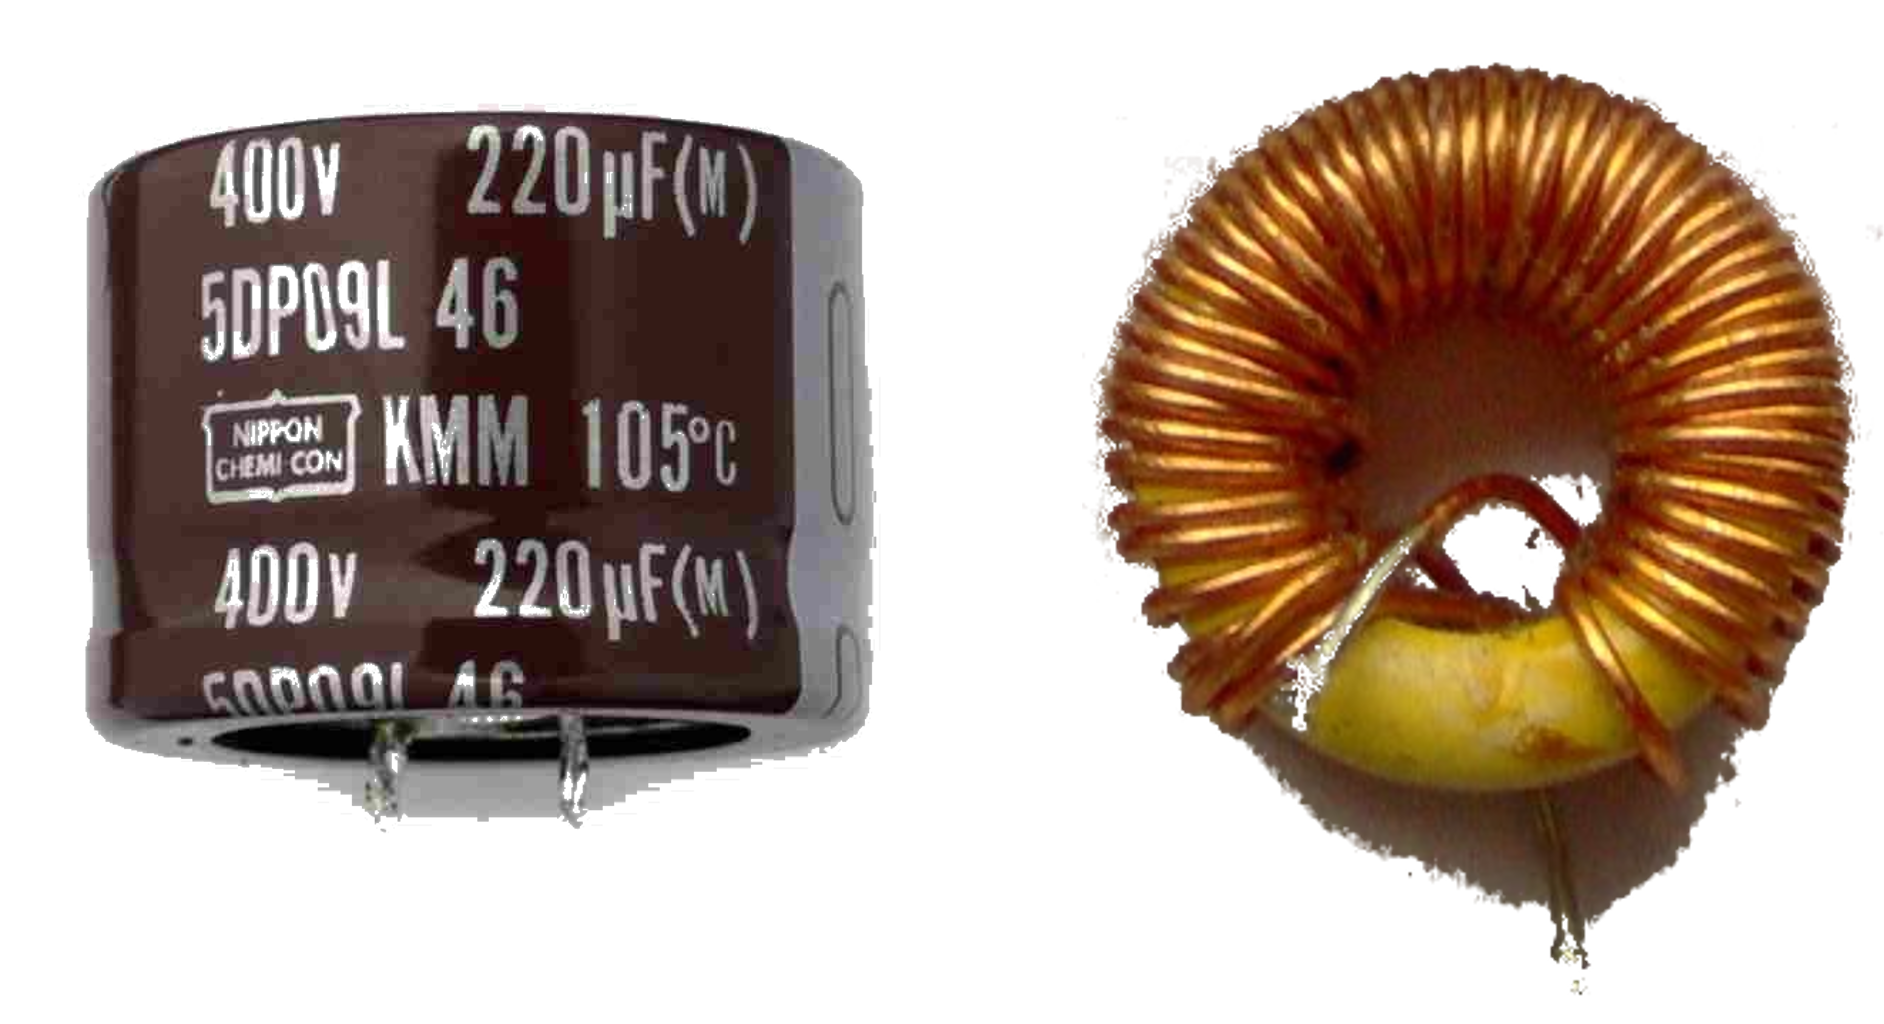
\includegraphics[scale=0.4]{KondensatorSpule/Bilder/KondensatorSpule.png}
 \vspace{-6cm}
\end{wrapfigure}

\section*{Theorie- und Prüfungsfragen} 


\mucho{1}{TC204}
{Wie verhält sich der Wechselstromwiderstand eines Kondensators mit zunehmender Frequenz?}%Frage
{Er bleibt konstant.}%A
{Er nimmt zu.}%B
{Er nimmt ab.}%C
{Er wird unendlich.}%D
{C}%Lösung

\mucho{2}{TC205}
{Wie groß ist der kapazitive Widerstand eines 10-pF-Kondensators bei 100 MHz?}%Frage
{31,8 $\Omega$}%A
{159 $\Omega$}%B
{318 $\Omega$}%C
{1,58 $k\Omega$}%D
{B}%Lösung

\mucho{3}{TC203}
{Ein verlustloser Kondensator wird an eine Wechselspannungsquelle angeschlossen. Welche Phasenverschiebung zwischen Spannung und Strom stellt sich ein?}%Frage
{Die Spannung eilt dem Strom um 45$^\circ$ voraus.}%A
{Der Strom eilt der Spannung um 45$^\circ$ voraus.}%B
{Der Strom eilt der Spannung um 90$^\circ$ voraus.}%C
{Die Spannung eilt dem Strom um 90$^\circ$ voraus.
}%D
{C}%Lösung

\mucho{4}{TC207}
{Was versteht man unter dem Blindwiderstand eines Kondensators und von welchen physikalischen Größen hängt er ab?}%Frage
{Der Blindwiderstand ist der Wechselstromwiderstand eines Kondensators. Er ist abhängig von der Kapazität des Kondensators und der anliegenden Frequenz. Im Blindwiderstand entstehen keine Wärmeverluste.}%A
{Der Blindwiderstand ist der Gleichstromwiderstand eines Kondensators. Er ist abhängig vom Isolationsmaterial des Kondensators und der anliegenden Spannung. Auch im Blindwiderstand entstehen Wärmeverluste.}%B
{Der Blindwiderstand ist der Wechselstromwiderstand eines Kondensators. Er ist abhängig von der Blindkapazität des Kondensators und der anliegenden Spannung. Im Blindwiderstand entstehen hohe Verluste.}%C
{Der Blindwiderstand ist der HF-Gleichstromwiderstand eines Kondensators. Er wird mit steigender Kapazität sowie bei erhöhtem Wechselstromanteil und steigender Frequenz größer. Je höher die Frequenz umso eher wandern die Ladungen an die Plattenränder (Skin-Effekt).}%D
{A}%Lösung

\mucho{5}{TD103}
{Wie groß ist die Gesamtkapazität von drei parallel geschalteten Kondensatoren von 20$nF$, 0,03$\mu F$ und 15000$pF$?}%Frage
{0,650$\mu F$}%A
{650$nF$}%B
{0,065$\mu F$}%C
{650000 $pF$}%D
{C}%Lösung

\mucho{6}{TC310}
{Mit einem Schalenkern, dessen AL-Wert mit 250 angegeben ist, soll eine Spule mit einer Induktivität von 2$mH$ hergestellt werden. Wie groß ist die erforderliche Windungszahl?}%Frage
{3}%A
{53}%B
{89}%C
{2828}%D
{C}%Lösung


\mucho{7}{TC306}
{Was versteht man unter dem Blindwiderstand einer Spule und von welchen physikalischen Größen hängt er ab?}%Frage
{Der Blindwiderstand ist der Wechselstromwiderstand einer Spule. Er ist abhängig von der Induktivität der Spule und der anliegenden Frequenz. Im Blindwiderstand entstehen keine Wärmeverluste.}%A
{Der Blindwiderstand ist der Gleichstromwiderstand einer Spule. Er ist abhängig vom Isolationsmaterial der Spule und der anliegenden Spannung. Auch im Blindwiderstand entstehen Wärmeverluste.}%B
{Der Blindwiderstand ist der Wechselstromwiderstand einer Spule. Er ist abhängig von der Blindinduktivität der Spule und der anliegenden Spannung. Im Blindwiderstand entstehen hohe Verluste.}%C
{Der Blindwiderstand ist der HF-Gleichstromwiderstand einer Spule. Er wird mit steigender Induktivität sowie bei erhöhtem Wechselstromanteil und steigender Frequenz größer. Je tiefer die Frequenz umso eher wandern die Elektronen an den Spulenrand (Skin-Effekt).}%D
{A}%Lösung

\mucho{8}{TC305}
{Wie groß ist der Wechselstromwiderstand einer Spule mit 3$\mu H$ Induktivität bei einer Frequenz von 100 MHz?}%Frage
{1,9$\Omega$}%A
{942$\Omega$}%B
{1885$\Omega$}%C
{1885$k\Omega$}%D
{C}%Lösung

\mucho{9}{TC302}
{In einer reinen Induktivität, die an einer Wechselspannungsquelle angeschlossen ist, eilt der Strom der angelegten Spannung ...}%Frage
{um 90 $^\circ$ voraus.}%A
{um 90 $^\circ$ nach.}%B
{um 45 $^\circ$ voraus.}%C
{um 45 $^\circ$ nach.}%D
{B}%Lösung


\chapter{Die Diode}


\begin{wrapfigure}[0]{r}[-2cm]{4cm}
 \vspace{-5cm}
 %\centering 
 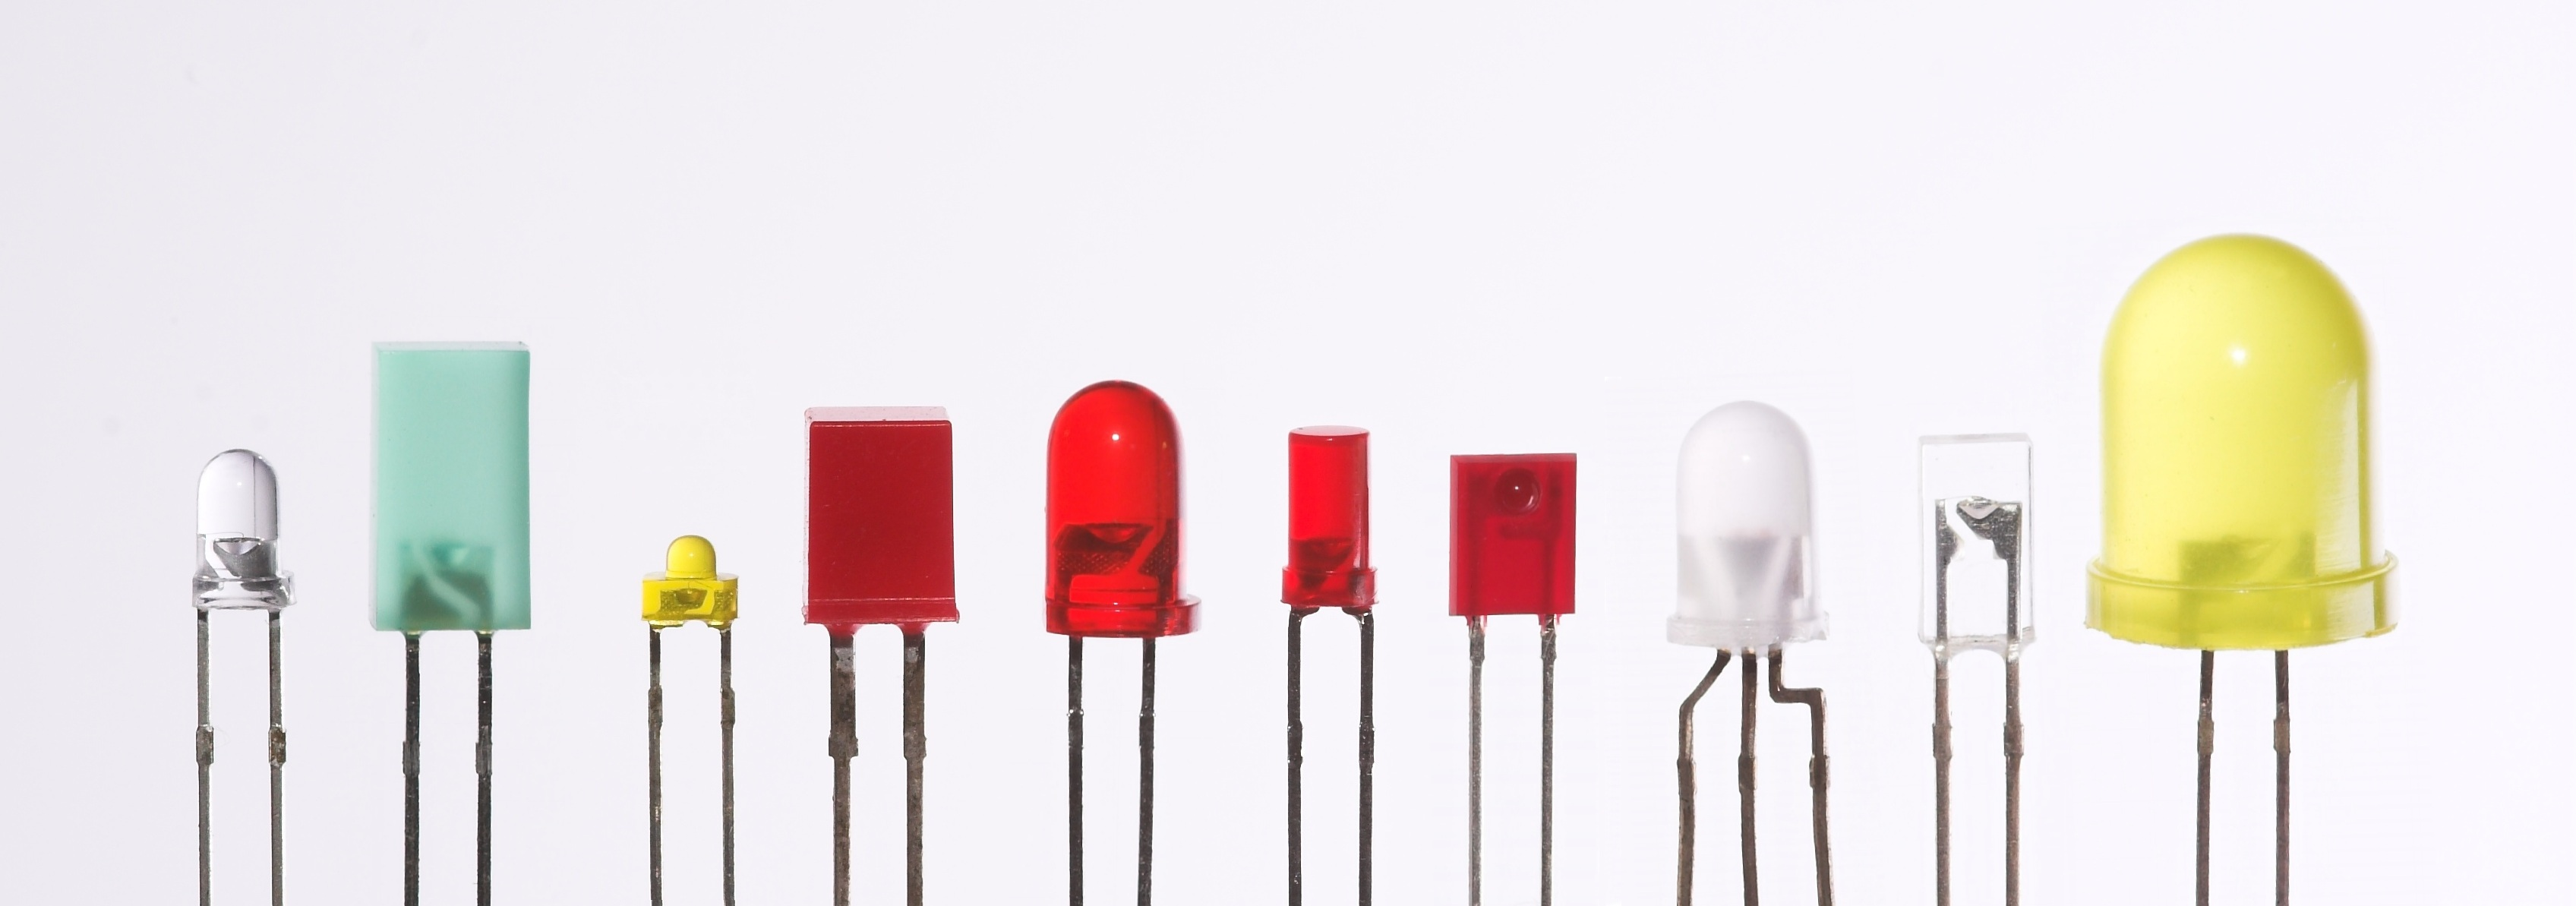
\includegraphics[scale=0.25]{Diode/Bilder/Verschiedene_LEDs.jpg}
 %\caption{Bildunterschrift der Grafik.}
 %\label{fig:meine-Grafik}
 \vspace*{-5cm}
\end{wrapfigure}


\section*{Theorie- und Prüfungsfragen} 

\subsection*{Dotierung}

\begin{enumerate}
	\itemsep1pt\parskip0pt\parsep0pt
	\item[1] Was bedeutet der Begriff Dotierung?
        \loesung{\textbf{Dotierung} bezeichnet in der Halbleitertechnik das
        einbringen von Fremdatomen in ein Grundmaterial zur Veränderung der
        elektrischen Leitfähigkeit.}
\end{enumerate}

\begin{enumerate}
\item[2] \emph{\textbf{TB105}}    Was verstehen Sie unter Halbleitermaterialien? Einige Stoffe wie z.B. ...
	\begin{enumerate}
	\itemsep1pt\parskip0pt\parsep0pt
		\item[A] Silizium, Germanium sind in reinem Zustand gute Isolatoren. Durch geringfügige Zusätze von geeigneten anderen Stoffen werden sie jedoch zu Leitern.
		\item[B] Silizium, Germanium sind in reinem Zustand gute Isolatoren. Durch geringfügige Zusätze von geeigneten anderen Stoffen nimmt jedoch ihre Leitfähigkeit ab.
		\item[C]  Indium oder Magnesium sind in reinem Zustand gute Isolatoren. Durch geringfügige Zusätze von geeigneten anderen Stoffen werden sie jedoch zu Leitern.
		\item[D] Silizium, Germanium sind in trockenem Zustand gute Elektrolyten. Durch geringfügige Zusätze von Wismut oder Tellur kann man daraus entweder N-leitendes oder P-leitendes Material für Anoden bzw. Katoden von Halbleiterbauelementen herstellen.
		\loesung{Lösung A}
	\end{enumerate}
\end{enumerate}

\begin{enumerate}
\item[3] \emph{\textbf{TC501}}    P-dotiertes Halbleitermaterial ist solches, das mit einem zusätzlichen Stoff versehen wurde, der
	\begin{enumerate}
	\itemsep1pt\parskip0pt\parsep0pt
		\item[A] mehr als vier Valenzelektronen enthält.
		\item[B] genau vier Valenzelektronen enthält.
		\item[C] weniger als vier Valenzelektronen enthält.
		\item[D] keine Valenzelektronen enthält.
		 \loesung{Lösung C}
	\end{enumerate}
\end{enumerate}


\begin{enumerate}
\item[4] \emph{\textbf{TC502}}   N-leitendes Halbleitermaterial ist gekennzeichnet durch
	\begin{enumerate}
	\itemsep1pt\parskip0pt\parsep0pt
		\item[A] Überschuss an freien Elektronen.
		\item[B] das Fehlen von Dotierungsatomen.
		\item[C] das Fehlen von Atomen im Gitter des Halbleiterkristalls.
		\item[D] bewegliche Elektronenlücken.
		\loesung{Lösung A}
	\end{enumerate}
\end{enumerate}


\begin{enumerate}
\item[5] \emph{\textbf{TC503}}  Ein in Durchlassrichtung betriebener PN-Übergang ermöglicht
	\begin{enumerate}
	\itemsep1pt\parskip0pt\parsep0pt
		\item[A] den Stromfluss von N nach P.
		\item[B] den Stromfluss von P nach N.
		\item[C] keinen Stromfluss.
		\item[D] den Elektronenfluss von P nach N.
		\loesung{Lösung B}
	\end{enumerate}
\end{enumerate}


\subsection*{Die Diode}

\begin{enumerate}
\itemsep1pt\parskip0pt\parsep0pt
\item[6] Skizziere das Schaltzeichen einer Diode und markiere die Anode, die Kathode und die jeweilige Dotierung.
    \loesung{
    \begin{figure}[H]
    \centering 
    % Graphic for TeX using PGF
% Title: /home/stole/Dokumente/git/afutub-kurs/Praxisskript/Diode/Schaltungen/Diode.dia
% Creator: Dia v0.97.3
% CreationDate: Mon Nov 16 20:36:17 2015
% For: stole
% \usepackage{tikz}
% The following commands are not supported in PSTricks at present
% We define them conditionally, so when they are implemented,
% this pgf file will use them.
\ifx\du\undefined
  \newlength{\du}
\fi
\setlength{\du}{15\unitlength}
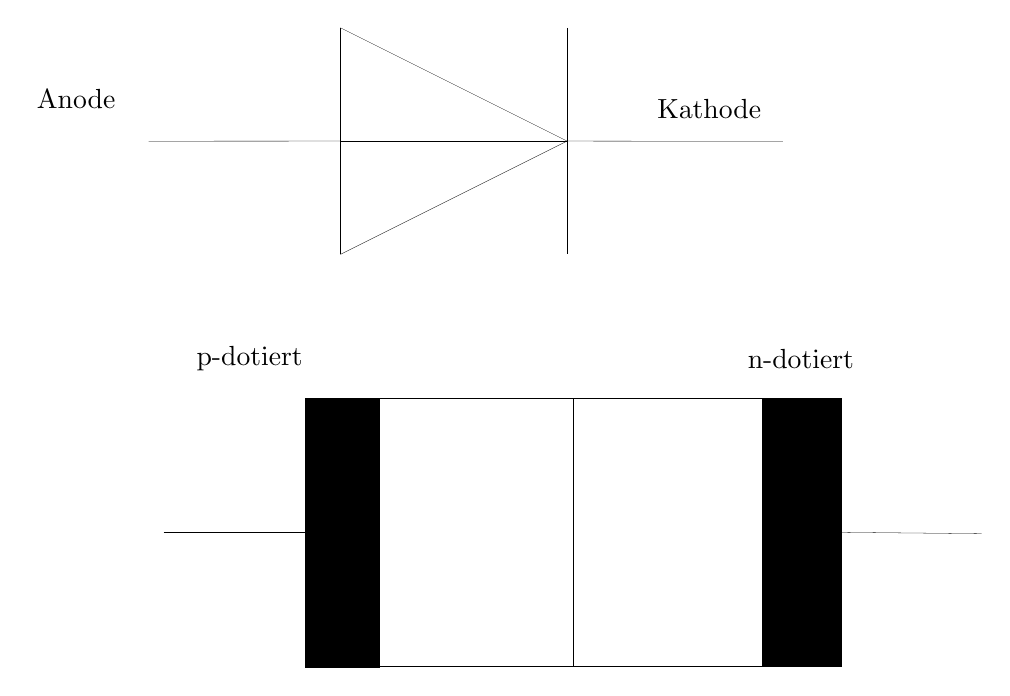
\begin{tikzpicture}
\pgftransformxscale{1.000000}
\pgftransformyscale{-1.000000}
\definecolor{dialinecolor}{rgb}{0.000000, 0.000000, 0.000000}
\pgfsetstrokecolor{dialinecolor}
\definecolor{dialinecolor}{rgb}{1.000000, 1.000000, 1.000000}
\pgfsetfillcolor{dialinecolor}
\pgfsetlinewidth{0.100000\du}
\pgfsetdash{}{0pt}
\pgfsetdash{}{0pt}
\pgfsetbuttcap
\pgfsetmiterjoin
\pgfsetbuttcap
\pgfsetmiterjoin
\pgfsetdash{}{0pt}
\definecolor{dialinecolor}{rgb}{0.000000, 0.000000, 0.000000}
\pgfsetstrokecolor{dialinecolor}
\draw (15.422302\du,-15.899999\du)--(15.422302\du,-13.022298\du);
\pgfsetbuttcap
\pgfsetmiterjoin
\pgfsetdash{}{0pt}
\definecolor{dialinecolor}{rgb}{0.000000, 0.000000, 0.000000}
\pgfsetstrokecolor{dialinecolor}
\draw (15.422302\du,-13.022298\du)--(18.300002\du,-14.461149\du);
\pgfsetbuttcap
\pgfsetmiterjoin
\pgfsetdash{}{0pt}
\definecolor{dialinecolor}{rgb}{0.000000, 0.000000, 0.000000}
\pgfsetstrokecolor{dialinecolor}
\draw (15.422302\du,-15.899999\du)--(18.300002\du,-14.461149\du);
\pgfsetbuttcap
\pgfsetmiterjoin
\pgfsetdash{}{0pt}
\definecolor{dialinecolor}{rgb}{0.000000, 0.000000, 0.000000}
\pgfsetstrokecolor{dialinecolor}
\draw (15.422302\du,-14.461149\du)--(18.300002\du,-14.461149\du);
\pgfsetbuttcap
\pgfsetmiterjoin
\pgfsetdash{}{0pt}
\definecolor{dialinecolor}{rgb}{0.000000, 0.000000, 0.000000}
\pgfsetstrokecolor{dialinecolor}
\draw (18.300002\du,-15.899999\du)--(18.300002\du,-13.022298\du);
\pgfsetlinewidth{0.100000\du}
\pgfsetdash{}{0pt}
\pgfsetdash{}{0pt}
\pgfsetbuttcap
{
\definecolor{dialinecolor}{rgb}{0.000000, 0.000000, 0.000000}
\pgfsetfillcolor{dialinecolor}
% was here!!!
\definecolor{dialinecolor}{rgb}{0.000000, 0.000000, 0.000000}
\pgfsetstrokecolor{dialinecolor}
\draw (18.300002\du,-14.461149\du)--(21.040301\du,-14.459230\du);
}
\pgfsetlinewidth{0.100000\du}
\pgfsetdash{}{0pt}
\pgfsetdash{}{0pt}
\pgfsetbuttcap
{
\definecolor{dialinecolor}{rgb}{0.000000, 0.000000, 0.000000}
\pgfsetfillcolor{dialinecolor}
% was here!!!
\definecolor{dialinecolor}{rgb}{0.000000, 0.000000, 0.000000}
\pgfsetstrokecolor{dialinecolor}
\draw (12.987653\du,-14.460276\du)--(15.422302\du,-14.461149\du);
}
% setfont left to latex
\definecolor{dialinecolor}{rgb}{0.000000, 0.000000, 0.000000}
\pgfsetstrokecolor{dialinecolor}
\node[anchor=west] at (11.448825\du,-14.995418\du){Anode};
% setfont left to latex
\definecolor{dialinecolor}{rgb}{0.000000, 0.000000, 0.000000}
\pgfsetstrokecolor{dialinecolor}
\node[anchor=west] at (19.327825\du,-14.872736\du){Kathode};
\pgfsetlinewidth{0.100000\du}
\pgfsetdash{}{0pt}
\pgfsetdash{}{0pt}
\pgfsetmiterjoin
\definecolor{dialinecolor}{rgb}{1.000000, 1.000000, 1.000000}
\pgfsetfillcolor{dialinecolor}
\fill (14.976770\du,-11.192971\du)--(14.976770\du,-7.792972\du)--(18.376770\du,-7.792972\du)--(18.376770\du,-11.192971\du)--cycle;
\definecolor{dialinecolor}{rgb}{0.000000, 0.000000, 0.000000}
\pgfsetstrokecolor{dialinecolor}
\draw (14.976770\du,-11.192971\du)--(14.976770\du,-7.792972\du)--(18.376770\du,-7.792972\du)--(18.376770\du,-11.192971\du)--cycle;
\pgfsetlinewidth{0.100000\du}
\pgfsetdash{}{0pt}
\pgfsetdash{}{0pt}
\pgfsetmiterjoin
\definecolor{dialinecolor}{rgb}{1.000000, 1.000000, 1.000000}
\pgfsetfillcolor{dialinecolor}
\fill (18.376770\du,-11.192970\du)--(18.376770\du,-7.792971\du)--(21.776770\du,-7.792971\du)--(21.776770\du,-11.192970\du)--cycle;
\definecolor{dialinecolor}{rgb}{0.000000, 0.000000, 0.000000}
\pgfsetstrokecolor{dialinecolor}
\draw (18.376770\du,-11.192970\du)--(18.376770\du,-7.792971\du)--(21.776770\du,-7.792971\du)--(21.776770\du,-11.192970\du)--cycle;
\pgfsetlinewidth{0.100000\du}
\pgfsetdash{}{0pt}
\pgfsetdash{}{0pt}
\pgfsetbuttcap
{
\definecolor{dialinecolor}{rgb}{0.000000, 0.000000, 0.000000}
\pgfsetfillcolor{dialinecolor}
% was here!!!
\definecolor{dialinecolor}{rgb}{0.000000, 0.000000, 0.000000}
\pgfsetstrokecolor{dialinecolor}
\draw (13.176770\du,-9.492971\du)--(14.976770\du,-9.492972\du);
}
\pgfsetlinewidth{0.100000\du}
\pgfsetdash{}{0pt}
\pgfsetdash{}{0pt}
\pgfsetmiterjoin
\definecolor{dialinecolor}{rgb}{0.000000, 0.000000, 0.000000}
\pgfsetfillcolor{dialinecolor}
\fill (14.976770\du,-11.192971\du)--(14.976770\du,-7.778107\du)--(15.911899\du,-7.778107\du)--(15.911899\du,-11.192971\du)--cycle;
\definecolor{dialinecolor}{rgb}{0.000000, 0.000000, 0.000000}
\pgfsetstrokecolor{dialinecolor}
\draw (14.976770\du,-11.192971\du)--(14.976770\du,-7.778107\du)--(15.911899\du,-7.778107\du)--(15.911899\du,-11.192971\du)--cycle;
\pgfsetlinewidth{0.100000\du}
\pgfsetdash{}{0pt}
\pgfsetdash{}{0pt}
\pgfsetmiterjoin
\definecolor{dialinecolor}{rgb}{0.000000, 0.000000, 0.000000}
\pgfsetfillcolor{dialinecolor}
\fill (20.776770\du,-11.192971\du)--(20.776770\du,-7.792971\du)--(21.776770\du,-7.792971\du)--(21.776770\du,-11.192971\du)--cycle;
\definecolor{dialinecolor}{rgb}{0.000000, 0.000000, 0.000000}
\pgfsetstrokecolor{dialinecolor}
\draw (20.776770\du,-11.192971\du)--(20.776770\du,-7.792971\du)--(21.776770\du,-7.792971\du)--(21.776770\du,-11.192971\du)--cycle;
% setfont left to latex
\definecolor{dialinecolor}{rgb}{0.000000, 0.000000, 0.000000}
\pgfsetstrokecolor{dialinecolor}
\node[anchor=west] at (13.476772\du,-11.692970\du){p-dotiert};
% setfont left to latex
\definecolor{dialinecolor}{rgb}{0.000000, 0.000000, 0.000000}
\pgfsetstrokecolor{dialinecolor}
\node[anchor=west] at (20.476772\du,-11.692970\du){n-dotiert};
\pgfsetlinewidth{0.100000\du}
\pgfsetdash{}{0pt}
\pgfsetdash{}{0pt}
\pgfsetbuttcap
{
\definecolor{dialinecolor}{rgb}{0.000000, 0.000000, 0.000000}
\pgfsetfillcolor{dialinecolor}
% was here!!!
\definecolor{dialinecolor}{rgb}{0.000000, 0.000000, 0.000000}
\pgfsetstrokecolor{dialinecolor}
\draw (21.776770\du,-9.492971\du)--(23.565624\du,-9.475251\du);
}
\end{tikzpicture}

    \end{figure}
    }
\item[7] Skizziere die Strom-Spannungskennlinie und markieren den Durchlassbereich, den Sperrbereich und den Durchbruchbereich.
	\loesung{
	\begin{figure}[H]
    \centering 
    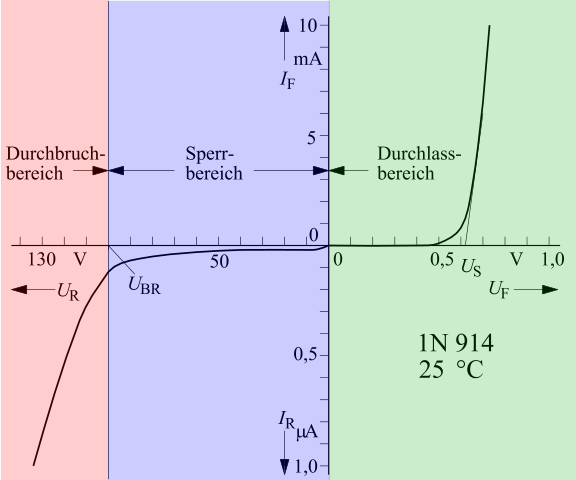
\includegraphics[scale=0.5]{Diode/Bilder/Kennlinie_Diode.png}
    \end{figure}
    }
\end{enumerate}

\mucho{8}{TC504}
{Eine in Sperrrichtung betriebene Diode hat}%Frage
{einen hohen Widerstand.}%A
{eine hohe Kapazität.}%B
{eine geringe Impedanz.}%C
{eine hohe Induktivität.}%D
{A}%Lösung

\mucho{9}{TC508}
{Wozu dient die folgende Schaltung?\\ 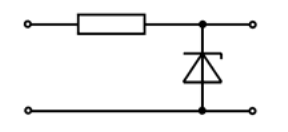
\includegraphics[scale=0.63]{Diode/Bilder/TC508.png}}%Frage
{zur Signalbegrenzung.}%A
{zur Spannungsstabilisierung.}%B
{als Leuchtanzeige.}%C
{zur Stromgewinnung.}%D
{B}%Lösung

\mucho{10}{TC505}
{Die Auswahlantworten enthalten Silizium-Dioden mit unterschiedlichen Arbeitspunkten. Bei welcher Antwort befindet sich die Diode in leitendem Zustand?}%Frage
{$-2,6V $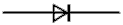
\includegraphics[scale=0.5]{Diode/Bilder/Diode_r.png} $-2,0V$}%A
{$~~~~15V$ 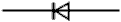
\includegraphics[scale=0.5]{Diode/Bilder/Diode_l.png} $~~~9V$}%B
{$~~0,7V$ 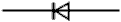
\includegraphics[scale=0.5]{Diode/Bilder/Diode_l.png} $1,3V$}%C
{$~~3,4V$ 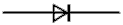
\includegraphics[scale=0.5]{Diode/Bilder/Diode_r.png} $4,0V$}%D
{C}%Lösung

\mucho{11}{TC506}
{Die Auswahlantworten enthalten Silizium-Dioden mit unterschiedlichen Arbeitspunkten. Bei welcher Antwort befindet sich die Diode in leitendem Zustand?}%Frage
{$~~5,3V $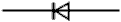
\includegraphics[scale=0.5]{Diode/Bilder/Diode_l.png} $4,7V$}%A
{$~~15V$ 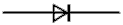
\includegraphics[scale=0.5]{Diode/Bilder/Diode_r.png} $18V$}%B
{$3,9V$ 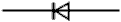
\includegraphics[scale=0.5]{Diode/Bilder/Diode_l.png} $3,2V$}%C
{$-2V$ 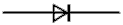
\includegraphics[scale=0.5]{Diode/Bilder/Diode_r.png} $-2,6V$}%D
{D}%Lösung

\mucho{12}{TC509}
{Wozu dient die folgende Schaltung?\\ 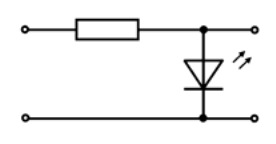
\includegraphics[scale=0.63]{Diode/Bilder/TC509.png}}%Frage
{zur Signalbegrenzung.}%A
{als Leuchtanzeige.}%B
{zur Stromgewinnung.}%C
{zur Spannungsstabilisierung.}%D
{B}%Lösung

\mucho{13}{TC507}
{Wie verhält sich die Kapazität einer Kapazitätsdiode (Varicap)?}%Frage
{Sie nimmt mit abnehmender Sperrspannung zu.}%A
{Sie erhöht sich mit zunehmender Durchlassspannung.}%B
{Sie nimmt mit zunehmender Sperrspannung zu.}%C
{Sie erhöht sich mit zunehmendem Durchlassstrom.}%D
{B}%Lösung


\chapter{Der Transistor}


\begin{wrapfigure}[2]{r}[-1cm]{4cm}
 \vspace{-6cm}
  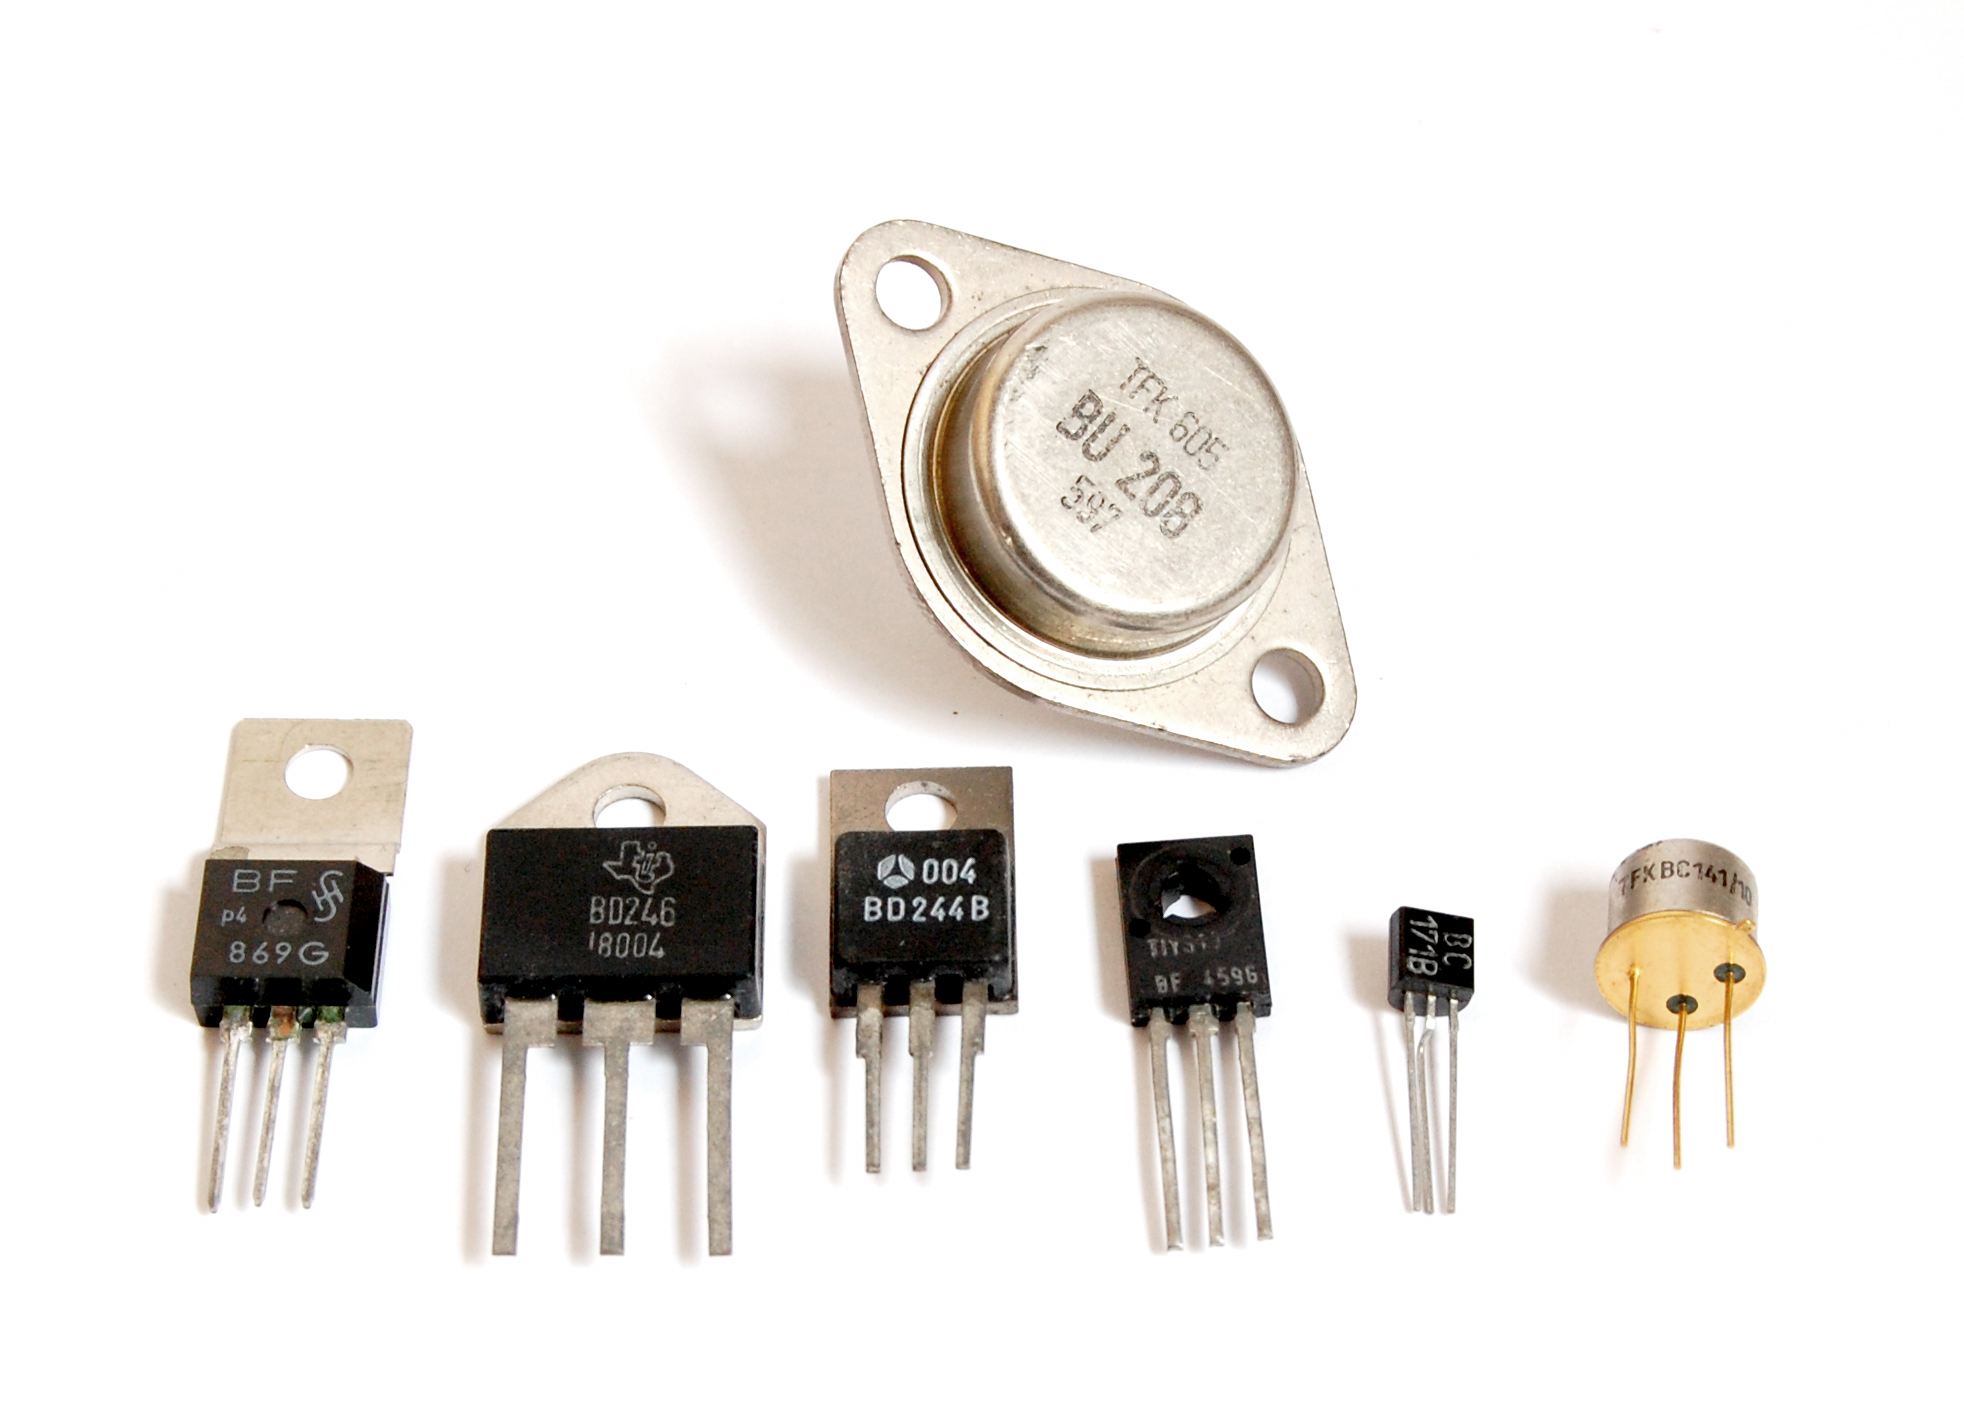
\includegraphics[scale=0.4]{Transistor/Bilder/Transistors-white.jpg}
 \vspace{-6cm}
\end{wrapfigure}

\section{Theorie- und Prüfungsfragen}

~~~~~~

\begin{enumerate}
\itemsep1pt\parskip0pt\parsep0pt
\item[i] Skizzieren Sie die Schaltzeichen eines NPN- und eines PNP-Transistors. Beschriften Sie entsprechend die Anschlüsse.
\item[ii] Zeichnen Sie das Ersatzschaltbild aus zwei Dioden für den NPN- und den PNP-Transistor.
\end{enumerate}

\begin{enumerate} 
\item[iii] \emph{\textbf{TC605}} Welche Kollektorspannungen haben NPN- und PNP-Transistoren?
	\begin{enumerate}
	\itemsep1pt\parskip0pt\parsep0pt
		\item[a] NPN- und PNP-Transistoren benötigen negative Kollektorspannungen.
		\item[b] PNP-Transistoren benötigen positive, NPN-Transistoren negative Kollektorspannung.
		\item[c] PNP- und NPN-Transistoren benötigen positive Kollektorspannungen.
		\item[d] NPN-Transistoren benötigen positive, PNP-Transistoren negative Kollektorspannungen.
	\end{enumerate}
\end{enumerate}

\loesung{	
	iii d
}

\begin{enumerate} 
\item[iv] \emph{\textbf{TC602}}  Das Verhältnis von Kollektorstrom zum Basisstrom eines Transistors liegt üblicherweise im Bereich von
	\begin{enumerate}
	\itemsep1pt\parskip0pt\parsep0pt
		\item[a] 1 zu 50 bis 1 zu 100.
		\item[b] 10 zu 1 bis 900 zu 1.
		\item[c] 1000 zu 1 bis 5000 zu 1.
		\item[d] 1 zu 100 bis 1 zu 500.
	\end{enumerate}
\end{enumerate}

\loesung{	
	iv b
}

\section{Praktische Anwendung}

\subsection[Der Bipolar-Transistor als Schalter]{Transistorschaltung 01 - Der Bipolar-Transistor als Schalter}

\begin{itemize}
\itemsep1pt\parskip0pt\parsep0pt
\item Schauen Sie sich den Bipolar-Transistor als Bauteil an und ordnen Sie die Bezeichnungen Kollektor, Basis und Emitter den einzelnen Beinchen zu.
\item Bauen Sie folgende Transistor-Schaltung auf (Abbildung \ref{s01}). 
\item Legen Sie die Versorgungsspannung an die Schaltung an.
\item Entfernen Sie unter Last die Leuchtdiode 1. Welche Auswirkungen hat das auf die Schaltung und warum?
\item \textbf{Zusatz:} Ersetzen Sie die Led durch einen Lautsprecher? Was passiert und warum?
\end{itemize}

\begin{figure}[H]
	\centering
	\subfigure[Schaltplan]{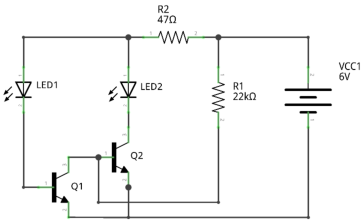
\includegraphics[scale=1.4]{Transistor/Schaltungen/NotBeleuchtung_Schaltplan.pdf}}
	\subfigure[Mögliche Breadboard-Ansicht]{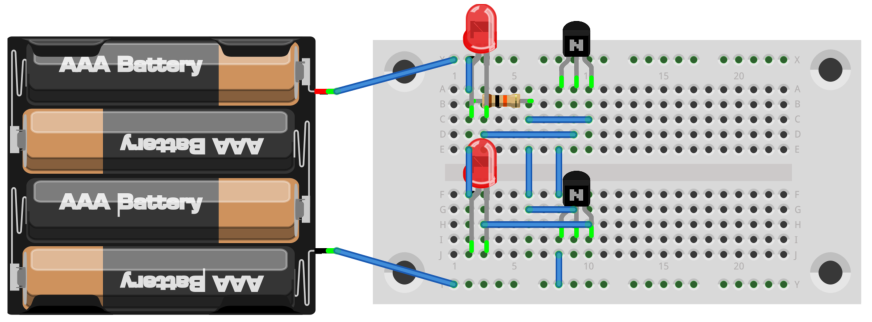
\includegraphics[scale=1]{Transistor/Schaltungen/NotBeleuchtung_Steckplatine.pdf}}
	\caption{Transistorschaltung 01 - Der Bipolar-Transistor als Schalter}
	\label{s01}
\end{figure}

%----------------------------------------------

\subsection[Der Bipolar-Transistor als Sensor]{Transistorschaltung 02 - Der Bipolar-Transistor als Sensor}

\begin{itemize}
\itemsep1pt\parskip0pt\parsep0pt
\item Bauen Sie folgende Transistor-Schaltung auf (Abbildung \ref{s02}). 
\item Legen Sie die Versorgungsspannung an die Schaltung an.
\item Berühren Sie die Basis des Transistors Q1 mit dem Finger. Was passiert und warum?
\end{itemize}

\begin{figure}[H]
	\centering
	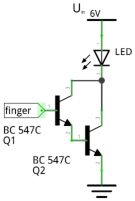
\includegraphics[scale=1.6]{Transistor/Schaltungen/NPN_Sensor.pdf}
	\caption{Transistorschaltung 02 - Der Bipolar-Transistor als Sensor}
	\label{s02}
\end{figure}

%----------------------------------------------

\subsection[Der Bipolar-Transistor als Verstärker]{Transistorschaltung 03 - Der Bipolar-Transistor als Verstärker}

\begin{itemize}
\itemsep1pt\parskip0pt\parsep0pt
\item Bauen Sie folgende Transistor-Schaltung auf (Abbildung \ref{s03}). 
\item Legen Sie die Versorgungsspannung an die Schaltung an.
\item Legen Sie ein Audiosignal an den Eingang der Schaltung an. Was passiert und warum?
\end{itemize}

\begin{figure}[H]
	\centering
	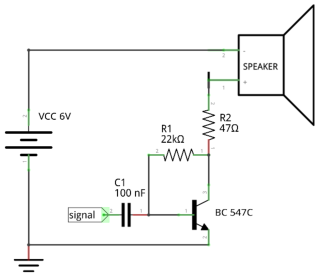
\includegraphics[scale=1.6]{Transistor/Schaltungen/NPN_Verstaerker.pdf}
	\caption{Transistorschaltung 03 - Der Bipolar-Transistor als Sensor}
	\label{s03}
\end{figure}

\chapter{Schwingkreis und Filter}
%\begin{wrapfigure}[0]{r}[-2.5cm]{3cm}
% \vspace{-6cm}
% \includegraphics[scale=0.4]{Schwingkreis/Bilder/schwingkreis.png}
% \vspace{-6cm}
%\end{wrapfigure}

\section*{Theorie- und Prüfungsfragen} 

\mucho{1}{TD203}
{Was ist im Resonanzfall bei der Reihenschaltung einer Induktivität mit einer Kapazität erfüllt?}%Frage
{Der Betrag des induktiven Widerstands ist dann gleich dem Betrag des kapazitiven Widerstands.}%A
{Der Wert des Verlustwiderstands der Spule ist dann gleich dem Wert des Verlustwiderstands des Kondensators.}%B
{Die Größe des elektrischen Feldes in der Spule ist dann gleich der Größe des elektrischen Feldes im Kondensators.}%C
{Die Größe des magnetischen Feldes in der Spule ist dann gleich der Größe des magnetischen Feldes im Kondensator.}%D
{A}%Lösung

\mucho{2}{TD209}
{Welche Resonanzfrequenz hat die Parallelschaltung einer Spule von 2 $\mu H$ mit einem Kondensator von 60 $pF$ und einem Widerstand von 10$k\Omega$?}%Frage
{145,288kHz}%A
{1,45288MHz}%B
{14,5288MHz}%C
{145,288 MHz}%D
{C \hspace{3em} $f_0 = \frac{1}{2 \pi \sqrt{L C}}$}%Lösung

\mucho{3}{TD206}
{ Wie ändert sich die Resonanzfrequenz eines Schwingkreises, wenn
1. die Spule mehr Windungen erhält, 2. die Länge der Spule durch Zusammenschieben der Drahtwicklung verringert wird, 3. ein Kupferkern in das Innere der Spule gebracht wird?}%Frage
{Die Resonanzfrequenz wird bei 1. und 2. kleiner und bei 3. größer.}%A
{Die Resonanzfrequenz wird in allen drei Fällen kleiner.}%B
{Die Resonanzfrequenz wird bei 1. kleiner und bei 2. und 3. größer.}%C
{Die Resonanzfrequenz wird bei 1. und 2. größer und bei 3. kleiner.}%D
{A}%Lösung


\mucho{4}{TD201}
{Der Impedanzfrequenzgang in der Abbildung zeigt die Kennlinie\\ 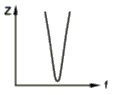
\includegraphics[scale=0.5]{Schwingkreis/Bilder/TD201.png}}%Frage
{eines Serienschwingkreises.}%A
{eines Parallelschwingkreises.}%B
{einer Induktivität.}%C
{einer Kapazität.}%D
{A}%Lösung

\vspace*{0.65cm}

\mucho{5}{TD202}
{Der Impedanzfrequenzgang in der Abbildung zeigt die Kennlinie\\
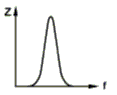
\includegraphics[scale=0.5]{Schwingkreis/Bilder/TD202.png}}%Frage
{eines Serienschwingkreises.}%A
{eines Parallelschwingkreises.}%B
{einer Induktivität.}%C
{einer Kapazität.}
{B}%Lösung

\aufgabentext{
	\begin{enumerate}
	\item[6] Um welche Schaltungen handelt es sich in folgender Abbildung.
	\end{enumerate}
	\loesung{1 Reihenschwingkreis, 2 Parallelschwingkreis, 3 Tiefpass, 4 Hochpass, 5 Bandpass, 6 Saugkreis, 7 Sperrkreis }
	}

\begin{figure}[H]
	\centering
	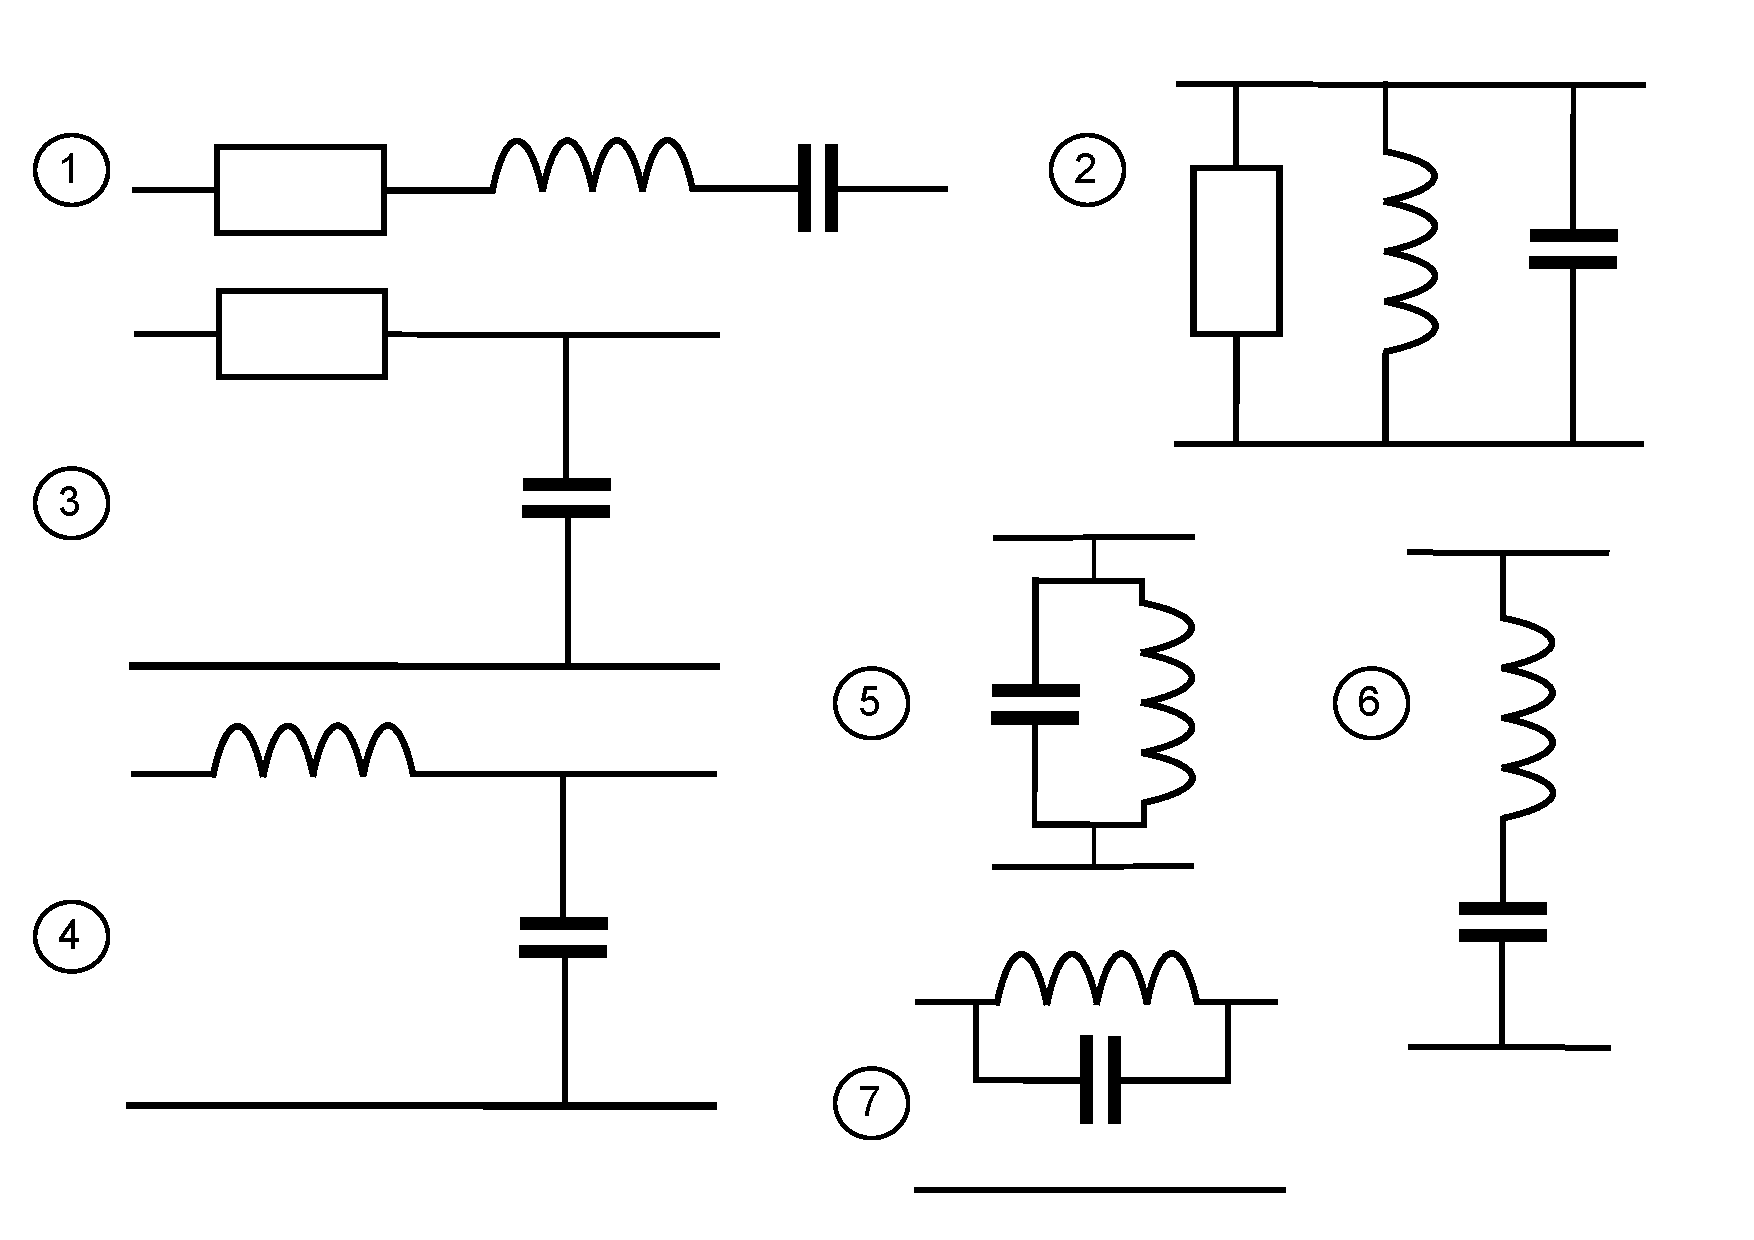
\includegraphics[scale=0.5]{Schwingkreis/Bilder/Filterschaltungen.pdf}
	\end{figure}

\mucho{7}{TD213}
{Welche Grenzfrequenz ergibt sich bei einem RC-Tiefpass mit einem Widerstand von 10$k\Omega$ und einem Kondensator von 50$nF$?}%Frage
{0,32$Hz$}%A
{318$Hz$}%B
{421$Hz$}%C
{318$kHz$}%D
{B \hspace{3em} $f_g = \frac{1}{2 \pi R C}$}%Lösung

\section*{Praxis}

\subsection*{Vorbereitung}

Seht euch die Pin-Belegung des Raspberry Pi (siehe Abbildung \ref{rpi}) sowie
die zu layoutende Schaltung für den 70cm-Tiefpassfilter (siehe Abbildung
\ref{70cmLP}) an.

\begin{figure}[H]
    \centering
    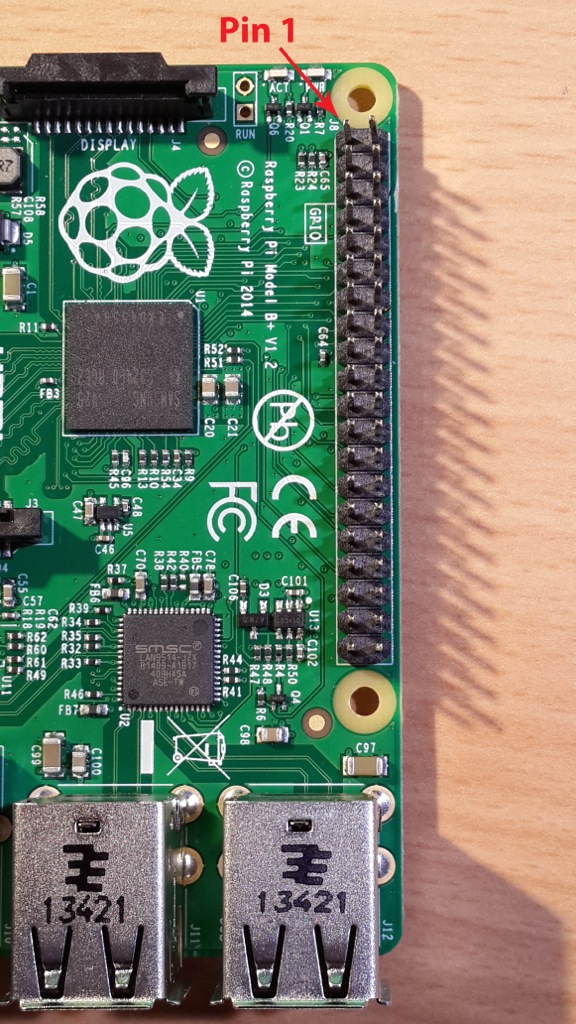
\includegraphics[height=0.4\textheight]{Schwingkreis/Bilder/B_plus_hdr_sm.jpg}
    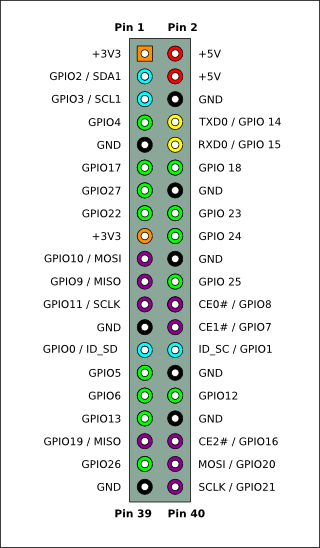
\includegraphics[height=0.4\textheight]{Schwingkreis/Bilder/Pi-GPIO-header.png}
    \caption{Connector pinout (P1 Header) -- Models B+, B2}
    \label{rpi}
    %FIXME Abbildungs-Quellenverzeichnis \url{http://elinux.org/RPi_Low-level_peripherals#Model_A.2B.2C_B.2B_and_B2}
\end{figure}

\begin{figure}[H]
    \centering
    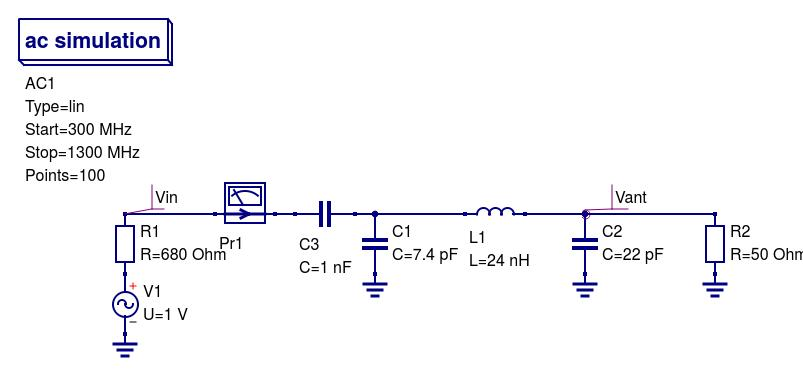
\includegraphics[width=1\textwidth]{Schwingkreis/Bilder/70cmLP500Ohm.jpg}
    \caption{Schaltung des 70cm-Tiefpassfilters aus Qucs}
    \label{70cmLP}
\end{figure}

\subsection*{Fritzing}

\subsubsection{Schematic View}

Bauteile aus den \emph{Core Parts} hinzufügen:

\begin{itemize}
    \item  Basic
    \begin{itemize}
        \item Resistor $680 \Omega$ (THT)
        \item Inductor $22 nH$ (SMD 1206)
        \item Ceramic Capacitor $1 nF$ (THT)
        \item Ceramic Capacitor $22 pF$ (THT)
    \end{itemize}
    \item  Input
    \begin{itemize}
        \item Variable Capacitor $2.1-10 pF$ (THT, $3.81mm$ pin spacing)
        \item Antenna (Wire soldering point)
    \end{itemize}
    \item Connection
    \begin{itemize}
        \item Generic female header (THT, 2x10, flip horizontal)
    \end{itemize}
    \item Schematic View
    \begin{itemize}
        \item Ground
    \end{itemize}
\end{itemize}

Nun können die Bauteile entsprechend des Schaltplanes verdrahtet werden.
\textbf{Hinweis}: Die Pin-Zählung des \emph{Generic female header} stimmt nicht
mit der des Raspberry Pi überein.

\begin{itemize}
    \item GPIO = Pin 16
    \item GND = Pin 17
\end{itemize}

\subsubsection{PCB View}

\begin{itemize}
    \item PCB ändern auf One Layer \& Fäche ca. $30x30mm$
    \item Bauteile anordnen (THT-Bauteile auf Vorderseite, SMD auf Unterseite)
    \item Leitungen ziehen
    \item optional: Copper Fill Blocker \& Silkscreen Text
    \item Rechtsklick auf einen Ground Pin: "`Set Ground Fill Seed"'
    \item Menü $\rightarrow$ Routing $\rightarrow$ Ground Fill
\end{itemize}

\subsubsection{Zusatzaufgaben}

\begin{itemize}
    \item Antennenanschluss auf folgende MCX-Buchse umbauen: \\
          \url{http://www.reichelt.de/index.html?ARTICLE=152523}
    \item Testboard mit verschiedenen PCB-Spulen um ~24 nH erstellen, da typ. 2-3\% Abweichung. \\
          Berechnungsgrundlagen mit Online calculator:\\
          \url{http://coil32.net/pcb-coil.html}\\
          alternative Formen: \\
          \url{http://www.circuits.dk/calculator_planar_coil_inductor.htm}
\end{itemize}


\chapter{Messtechnik}
\begin{wrapfigure}[0]{r}[-4cm]{3cm}
 \vspace{-6cm}
 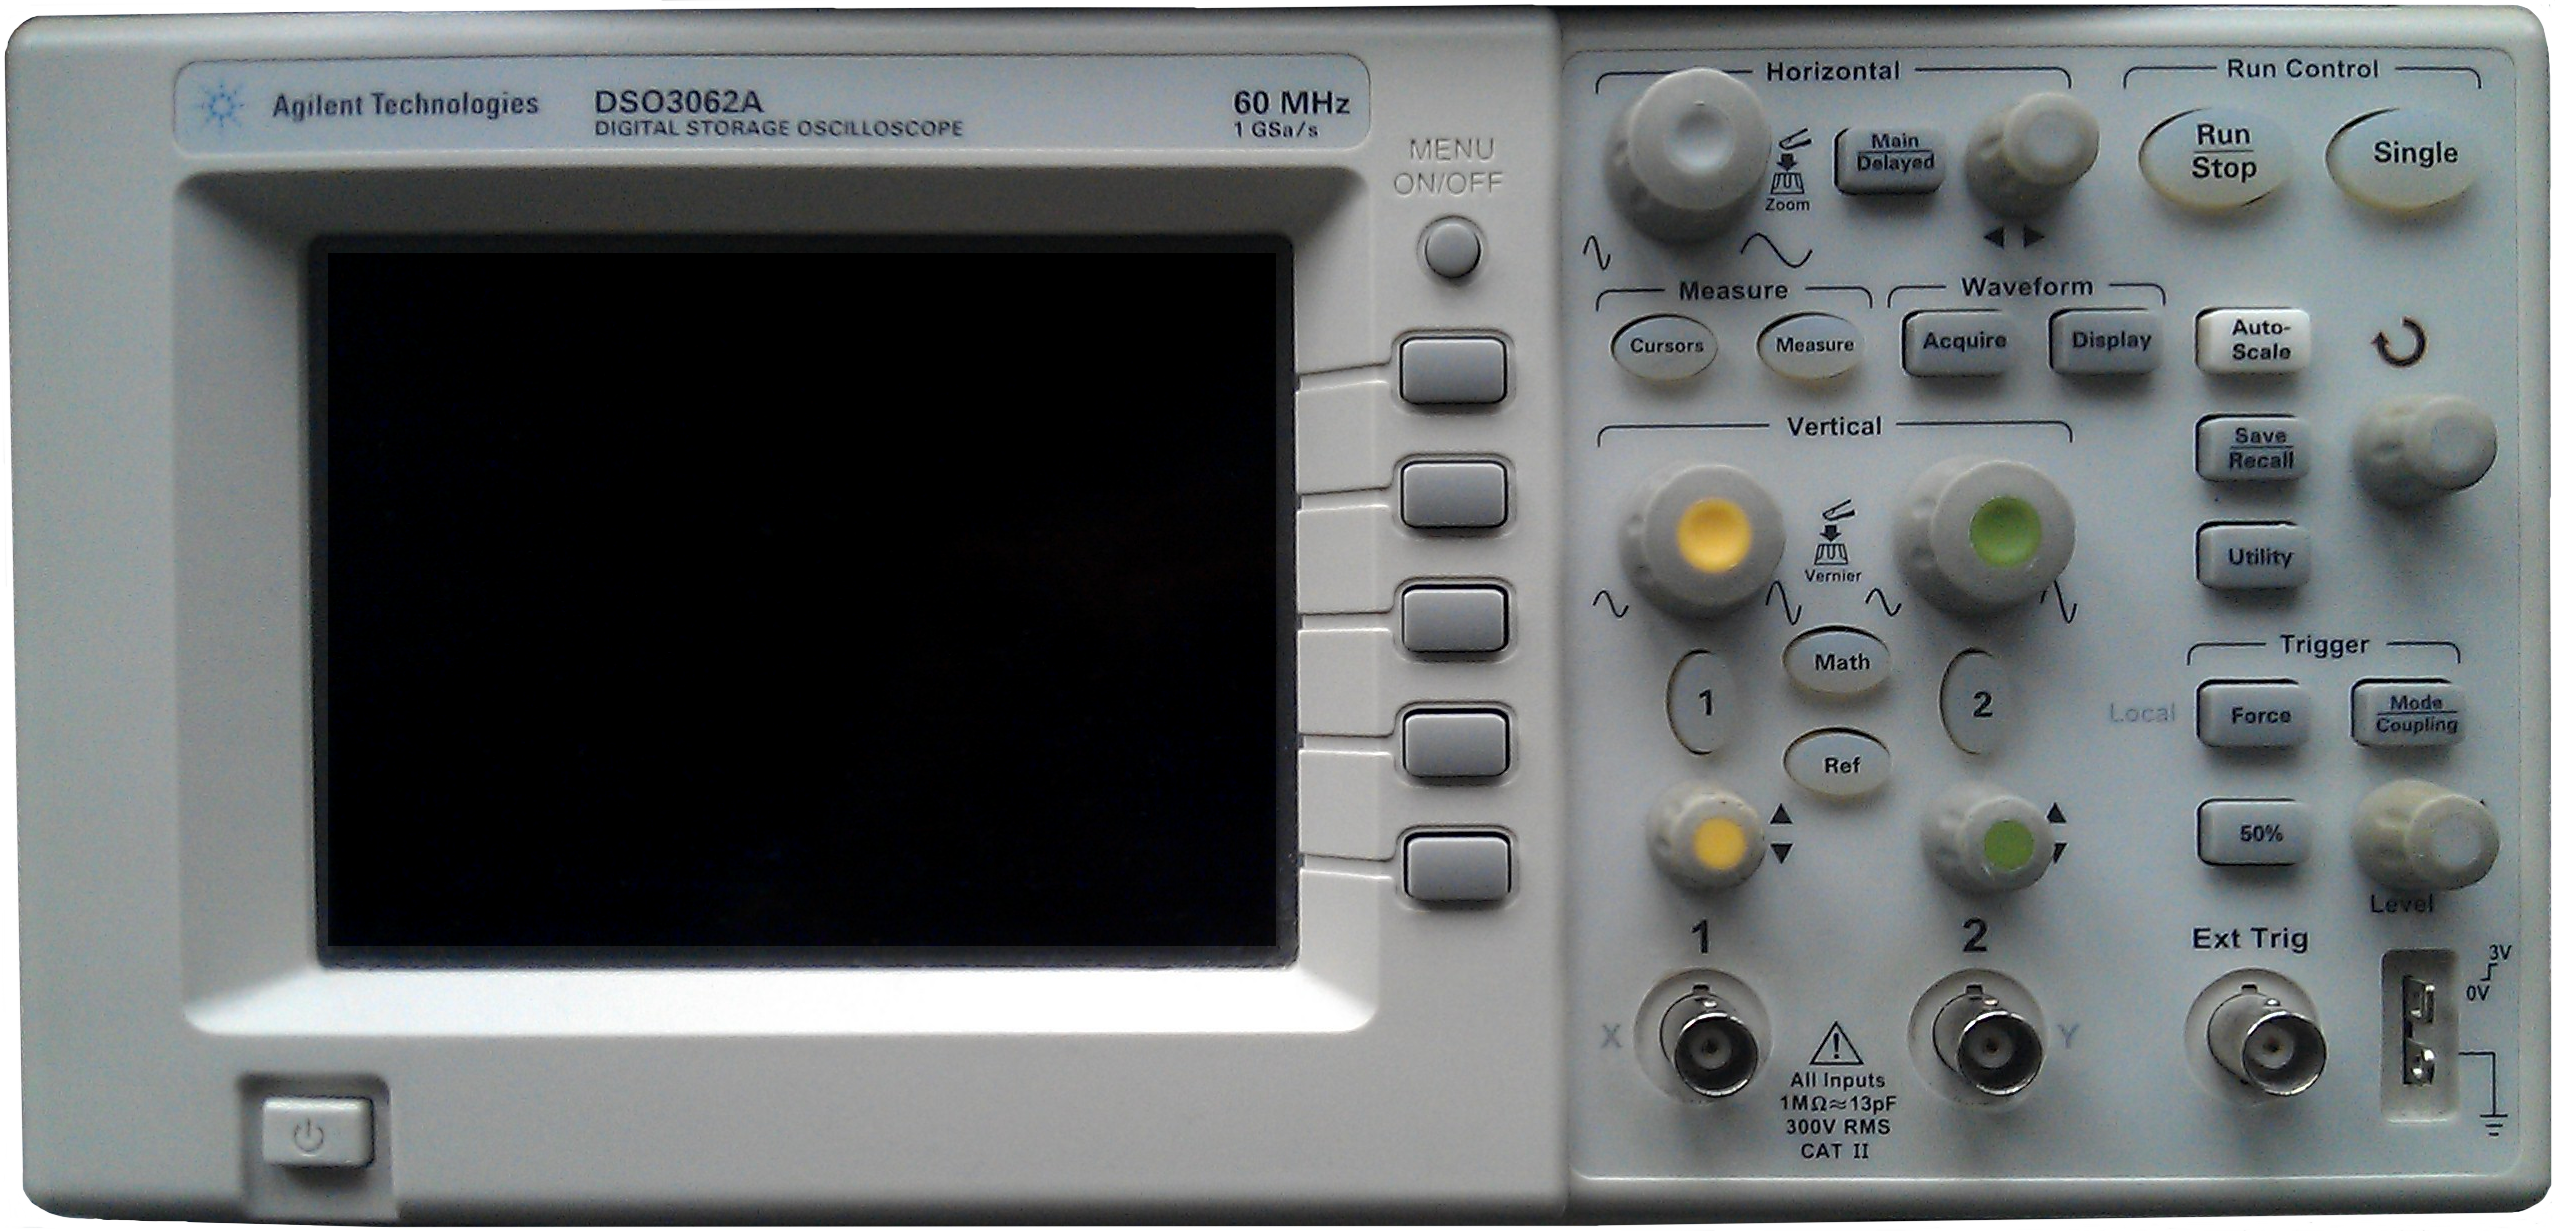
\includegraphics[scale=0.08]{Messtechnik/Bilder/oszi_foto.png}
 \vspace{-6cm}
\end{wrapfigure}

\section*{Theorie- und Prüfungsfragen} 

\mucho{1}{TJ101}
{Das Prinzip des Drespulmessgerätes berut auf}%Frage
{der Wechselwirkung der Kräfte zwischen zwei permanent magnetischen Feldern.}%A
{der Wechselwirkung der Kräfte zwischen einem magnetischen und einem elektrischen Feld.}%B
{der Wechselwirkung der Kräfte zwischen einem permanent magnetischen und einem elektromagentischen Feld.}%C
{dem erdmagentischen Feld.}%D
{C}%Lösung

\mucho{2}{TJ102}
{Das Drehspulmesswerk in der folgenden Schaltung hat einen maximalen Messstrom $I_M = 100\mu A$ und einen Messwerkwiderstand $R_M = 1 k\Omega$; $R_V = 499 k\Omega$. Welche Gleichspannung muss an die Gesamtschaltung angelegt werden, damit das Messwerk Vollausschlag anzeigt?\\
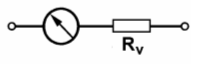
\includegraphics[scale=0.5]{Messtechnik/Bilder/TJ102.png}}%Frage
{10V}%A
{50V}%B
{500V}%C
{100V}%D
{B}%Lösung


\mucho{3}{TJ805}
{Mit einem Voltmeter der Klasse 1.5, das einen Skalenendwert von 300V hat, messen Sie an einer Spannungsquelle 230V. In welchem Bereich liegt der wahre Wert?}%Frage
{Er liegt zwischen 225,5 und 234,5V.}%A
{Er liegt zwischen 226,5 und 233,5V.}%B
{Er liegt zwischen 229,5 und 230,5V.}%C
{Er liegt zwischen 229,7 und 230,3V.}%D
{A \hspace{3em} Klasse 1.5 $\rightarrow 1,5\% \Rightarrow
                            300V \cdot 0,015 = 4,5V \Rightarrow \pm 4,5V$ }%Lösung


\mucho{4}{TJ115}
{Ein Drehspulmessgerät hat normalerweise eine Genauigkeit von}%Frage
{ca. 1,5 \% vom Endausschlag.}%A
{ca. 0,3 \% vom Ablesewert.}%B
{ca. 0,3 \% vom Endausschlag.}%C
{ca. 0,05 \% vom Ablesewert.}%D
{A}%Lösung

\mucho{5}{TG219}
{Die richtige Oberwellenauswahl in einer Vervielfachungsstufe lässt sich am leichtesten mit einem}%Frage
{Diodentastkopf prüfen.}%A
{Absorptionsfrequenzmesser prüfen.}%B
{Universalmessgerät prüfen.}%C
{Frequenzzähler prüfen.}%D
{B}%Lösung


\mucho{6}{TJ602}
{Ein Absorptionsfrequenzmesser hat normalerweise eine Genauigkeit von}%Frage
{1 \%.}%A
{5 \%. }%B
{0,05 \%.}%C
{0,001 \%.}%D
{B}%Lösung


\mucho{7}{TJ812}
{Wie ermittelt man die Resonanzfrequenz eines passiven Schwingkreises?}%Frage
{Durch Messung von L und C und Berechnung oder z.B. mit einem Dip-Meter.}%A
{Mit einem Frequenzmesser oder einem Oszilloskop.}%B
{Mit einem Digital-Multimeter in der Stellung Frequenzmessung.}%C
{Mit Hilfe der S-Meter Anzeige bei Anschluss des Schwingkreises an den Empfängereingang.}%D
{A}%Lösung

\mucho{8}{TJ206}
{Ein Dip-Meter hat normalerweise eine Genauigkeit von etwa}%Frage
{1 \%.}%A
{10 \%.}%B
{0,05 \%.}%C
{0,001 \%.}%D
{B}%Lösung

\mucho{9}{TJ501}
{Um die Skalenendwerte einer Sende-/Empfangsanlage mit VFO mit hinreichender Genauigkeit zu überprüfen, kann man}%Frage
{einen Frequenzzähler verwenden.}%A
{ein Dipmeter verwenden.}%B
{einen Absorptionsfrequenzmesser verwenden.}%C
{ein Oszilloskop verwenden.}%D
{A}%Lösung

\mucho{10}{TJ402}
{Für welchen Zweck wird eine Stehwellenmessbrücke verwendet?}%Frage
{Zur Überprüfung der Anpassung des Senders an die Antenne}%A
{zur Frequenzkontrolle.}%B
{zur Modulationskontrolle.}%C
{als Abschluss des Senders.}%D
{A}%Lösung

\mucho{11}{TJ305}
{Welches dieser Geräte wird für die Anzeige von NF-Verzerrungen verwendet?}%Frage
{Frequenzzähler}%A
{Transistorvoltmeter}%B
{Vielfachmessgerät}%C
{Oszilloskop}%D
{D}%Lösung

\mucho{12}{TJ303}
{Um auf dem Bildschirm eines Oszilloskops ein stehendes Bild statt durchlaufender Wellenzüge zu erhalten muss, das Oszilloskop}%Frage
{eine Triggereinrichtung haben.}%A
{einen X-Vorteiler haben.}%B
{einen Y-Vorteiler haben. \vspace*{-0.06cm}}%C
{einen Frequenzmarken-Generator haben.}%D
{A}%Lösung


\section*{Praxis}

\subsection*{PCB mit 30m-LPF: Bestücken \& Löten}

Bestückt und verlötet die Bauteile auf der 30m-Platine! Die Schaltung ist noch
einmal in Abbildung \ref{fig:30mLP} dargestellt. Beachtet den richtigen Einbau
des Transistors (CBE -- von der flachen Seite aus betrachtet) sowie beim Löten
des SMDs:

\begin{itemize}
    \item als erstes ein Lötpad etwas verzinnen
    \item Zinn erwärmen und das Bauteil mit einer Pinzette darauf ablegen
    \item wenn das Bauteil plan aufliegt, abschließend das andere Pad verlöten
\end{itemize}

% Berechnet eine einfache Groundplane-Antenne ($\lambda/4$) für das Band von $430
% MHz$ bis $440 MHz$ und schneidet die entsprechende Länge aus einem starren
% Draht. Dieser wird nun so auf das Antennenpad aufgelötet, dass die Antenne
% gegenüber von der Buchsenleiste steht -- sprich: auf der Leiterbahnseite.

% Baut einen weiteren Tiefpassfilter auf einer Lochrasterplatine auf. Beachtet,
% dass diesmal \textbf{TX via GPIO 4 (Pin 7)} und ein beliebiger GND verdrahtet
% werden muss (siehe Abbildung \ref{rpi}).

Die Spule dient später zum Abstimmen und soll von Hand auf einen $8
mm$-Durchmesser auf ca. $1 cm$ Länge gewickelt werden -- wieviele Windungen
müssen das sein? Teste das Resultat mit dem LC-Messgerät.

\textbf{Hinweis}: Als Vorwiderstand verbauen wir im Kurs $470 \Omega$ um unsere
\emph{Raspberry Pi}s gegen versehentliches Kurzschließen zu schützen. Später kann dieser
gegen einen geringeren Widerstand oder sogar eine Drahtbrücke ausgetauscht
werden, um mehr Leistung an der Antenne zu erhalten. Erklärung: Der Stromfluss
wird durch den Widerstand begrenzt ($I = \frac{U}{R} = \frac{3,3 V}{470 \Omega}
\approx 7 mA$). Mit $220 \Omega$ auf $15 mA$ sollte man aber auch noch auf der
sicheren Seite sein -- "`das Internet"' berichtet von $30 mA$ am GPIO ohne
bleibende Schäden. ;-) Ist sichergestellt, dass der Filter und die Abstrahlung
an der Antenne funktionieren, kann der Widerstand auch wie gesagt weggelassen
werden. \textbf{Frage:} Welche Leistungen ergeben sich je nach Vorwiderstand
ungefähr?

\loesung{$P = U \cdot I$ \\
         $7 mA$: $3,3 V \cdot 0.007 A \approx 23 mW$ \\
         $15 mA$: $3,3 V \cdot 0.015 A \approx 50 mW$ \\
         $30 mA$: $3,3 V \cdot 0.030 A \approx 100 mW$}

\begin{figure}[H]
    \centering
    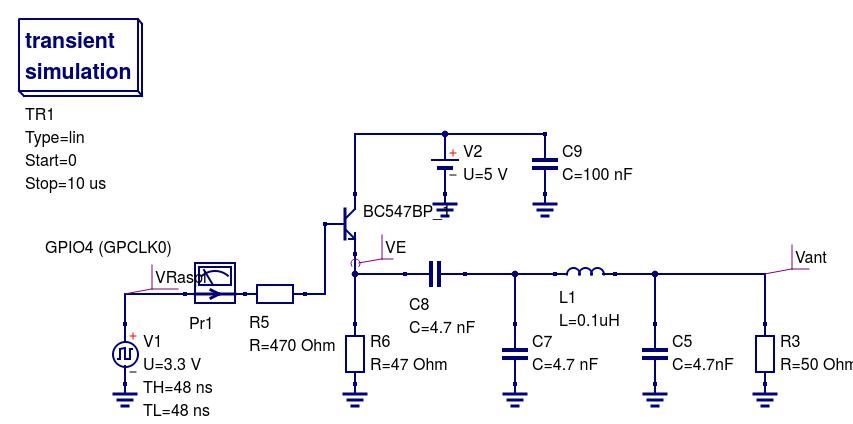
\includegraphics[width=0.9\textwidth]{Messtechnik/Bilder/30mRaspiAmpLP.jpg}
    \caption{Schaltung des 30m-Tiefpassfilters aus Qucs}
    \label{fig:30mLP}
\end{figure}

\subsection*{Kalibrierung}

Lege eine $5V$-Gleichspannung am Transistor an. Erzeuge mit dem
Frequenzgenerator am Eingang der Filterschaltung ein 10-MHz-Signal. Miss mit dem
Oszilloskop oder Spektrum-Analyzer oder RTL-SDR die Amplitude am Ausgang. Nun
wird das Filter durch Strecken oder Stauchen der Spule auf maximale
Ausgangsleistung abgestimmt.

\subsection*{Messprotokoll}

% FIXME Es fehlt eine Auswertung der Ergebnisse

\begin{enumerate}
% FIXME Nochmal Aufgabe umformulieren, durch die DC-Entkopplung tut sich natürlich nichts.
%      stole nochmal fragen, was er sich dabei gedacht hat.
% 	\item Das lineare Verhalten eines Tiefpassfilters.
% 		\begin{itemize}
% 			\item Nutze die Gleichspannungsquelle und das Tischmultimeter.
% 			\item Lege eine Gleichspannung an den Eingang des Tiefpassfilters und messe die Ausgangsspannung.
%     		\item Die Eingangspannung soll zwischen $-5~V$ und $+5~V$ liegen.
%     		\item Die Eingangsspannung soll in $2~V$-Schritten geändert werden.
%     		\item Um eine negative Gleichspannung mit der Gleichspannungsquelle zu realisieren, muss umgepolt werden.
%     		\item Miss mit Hilfe des Tischmultimeters die Ausgangsspannung des Tiefpassfilters (Siehe Abbildung \ref{block1}).
%     		\item Notiere die Messwerte direkt in Scilab, Octave oder einer Tabellekalkulation.
% 			\item Plotte den Verlauf der Ausgangsspannung in Abhängigkeit der Eingangsspannung.
% 			\item \textbf{Zusatz:} Plotte den idealen Kennlinienverlauf mit in den selben Plott.
% 			\end{itemize}	
	\item Das Messen des Amplitudenganges eines Tiefpassfilters mit Hilfe des Oszilloskops.
		\begin{itemize}
			\item Nutze den Frequenzgenerator und das Oszilloskop.
			\item Stelle am Frequenzgenerator ein Sinus-Signal mit einer Amplitude von
        $5~V$ ein und lege diese an den Eingang des Tiefpassfilters.
			\item Miss mit Hilfe des Oszilloskops die Eingangs- und die Ausgangsspannung des Tiefpassfilters (Siehe Abbildung \ref{block2}).
			\item Erhöhe schrittweise die Frequenz .
			\item Nimm insgesamt 20 Messwerte auf.
			\item Verteile die Messwerte über einen Bereich von $10^6~Hz$ bis $10^8~Hz$.
			\item Verwende \texttt{$V_{RMS}$} der \texttt{Measure}-Funktion zur Messung der Amplitude
			\item Notiere die Messwerte direkt in Scilab, Octave oder einer Tabellekalkulation.
			\item Plotte den Verlauf der Amplitude (Ausgangsspannung) in Abhängigkeit der Frequenz.
			\item \textbf{Zusatz:} Stelle die Amplitude in dB dar und stelle die X-Achse auf logarthmische Darstellung um.
			\end{itemize}
	\item Das Messen der Sprungantwort eines Tiefpassfilters.
		\begin{itemize}
			\item Nutze den Frequenzgenerator und das Oszilloskop.
        % FIXME hxb Richtige Rechteckfrequenz raussuchen, die durch den Koppel-C kommt
			\item Erzeuge mit dem Funktionsgenerator eine Rechteckfunktion mit einer Amplitude von $2,5~V$, mit einem Offset von $2,5 V$ und einer Frequenz von $5~Hz$ und lege diese an den Eingang des Tiefpassfilters.
			\item Miss mit Hilfe des Oszilloskops die Eingangs- und die Ausgangsspannung des Tiefpassfilters (Siehe Abbildung \ref{block2}).
			\item Übertrage die Sprungantwort ins Protokoll (Foto, Skizze).
			\item Hinweise zum Umgang mit dem Oszilloskop:
				\begin{itemize}
					\item Achte darauf, dass bei den einzelnen Kanälen (\textbf{CH1}, \textbf{CH2}) bei \textbf{Kopplung}: \textbf{DC} eingestellt ist.
					\item Um einwandfrei messen zu können, verwendet die Trigger-Funktion
            des Oszilloskops. Drückt die Taste \textbf{Mode/Coupling} in der
            Trigger-Sektion. Wählt beim oberen \textbf{Modus}: \textbf{Flanke}, bei \textbf{Quelle}: \textbf{CH2}, beim unteren \textbf{Modus}: \textbf{Normal} und bei der \textbf{Kopplung}: \textbf{AC} aus.
					\end{itemize}
			\end{itemize}
 	\end{enumerate} 

% \begin{figure}[H]
% 	\centering
% 	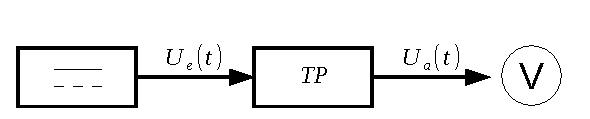
\includegraphics[scale=1]{Messtechnik/Bilder/Block_Messung_Kennlinie.pdf}
% 	\caption{Blockschaltbild für die Messungen mit dem Tischmultimeter.}
% 	\label{block1}
% \end{figure}

\bigskip

\begin{figure}[H]
	\centering
	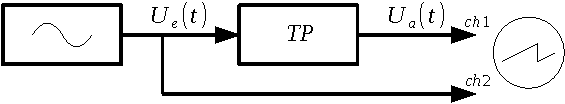
\includegraphics[scale=1]{Messtechnik/Bilder/Block_Messung_oszi.pdf}
	\caption{Blockschaltbild der Signalspannung für die Messungen mit dem Oszilloskop}
	\label{block2}
	\end{figure}


\chapter{Oszillator und Hochfrequenzverstärker}
%\begin{wrapfigure}[0]{r}[-4cm]{3cm}
% \vspace{-6cm}
% 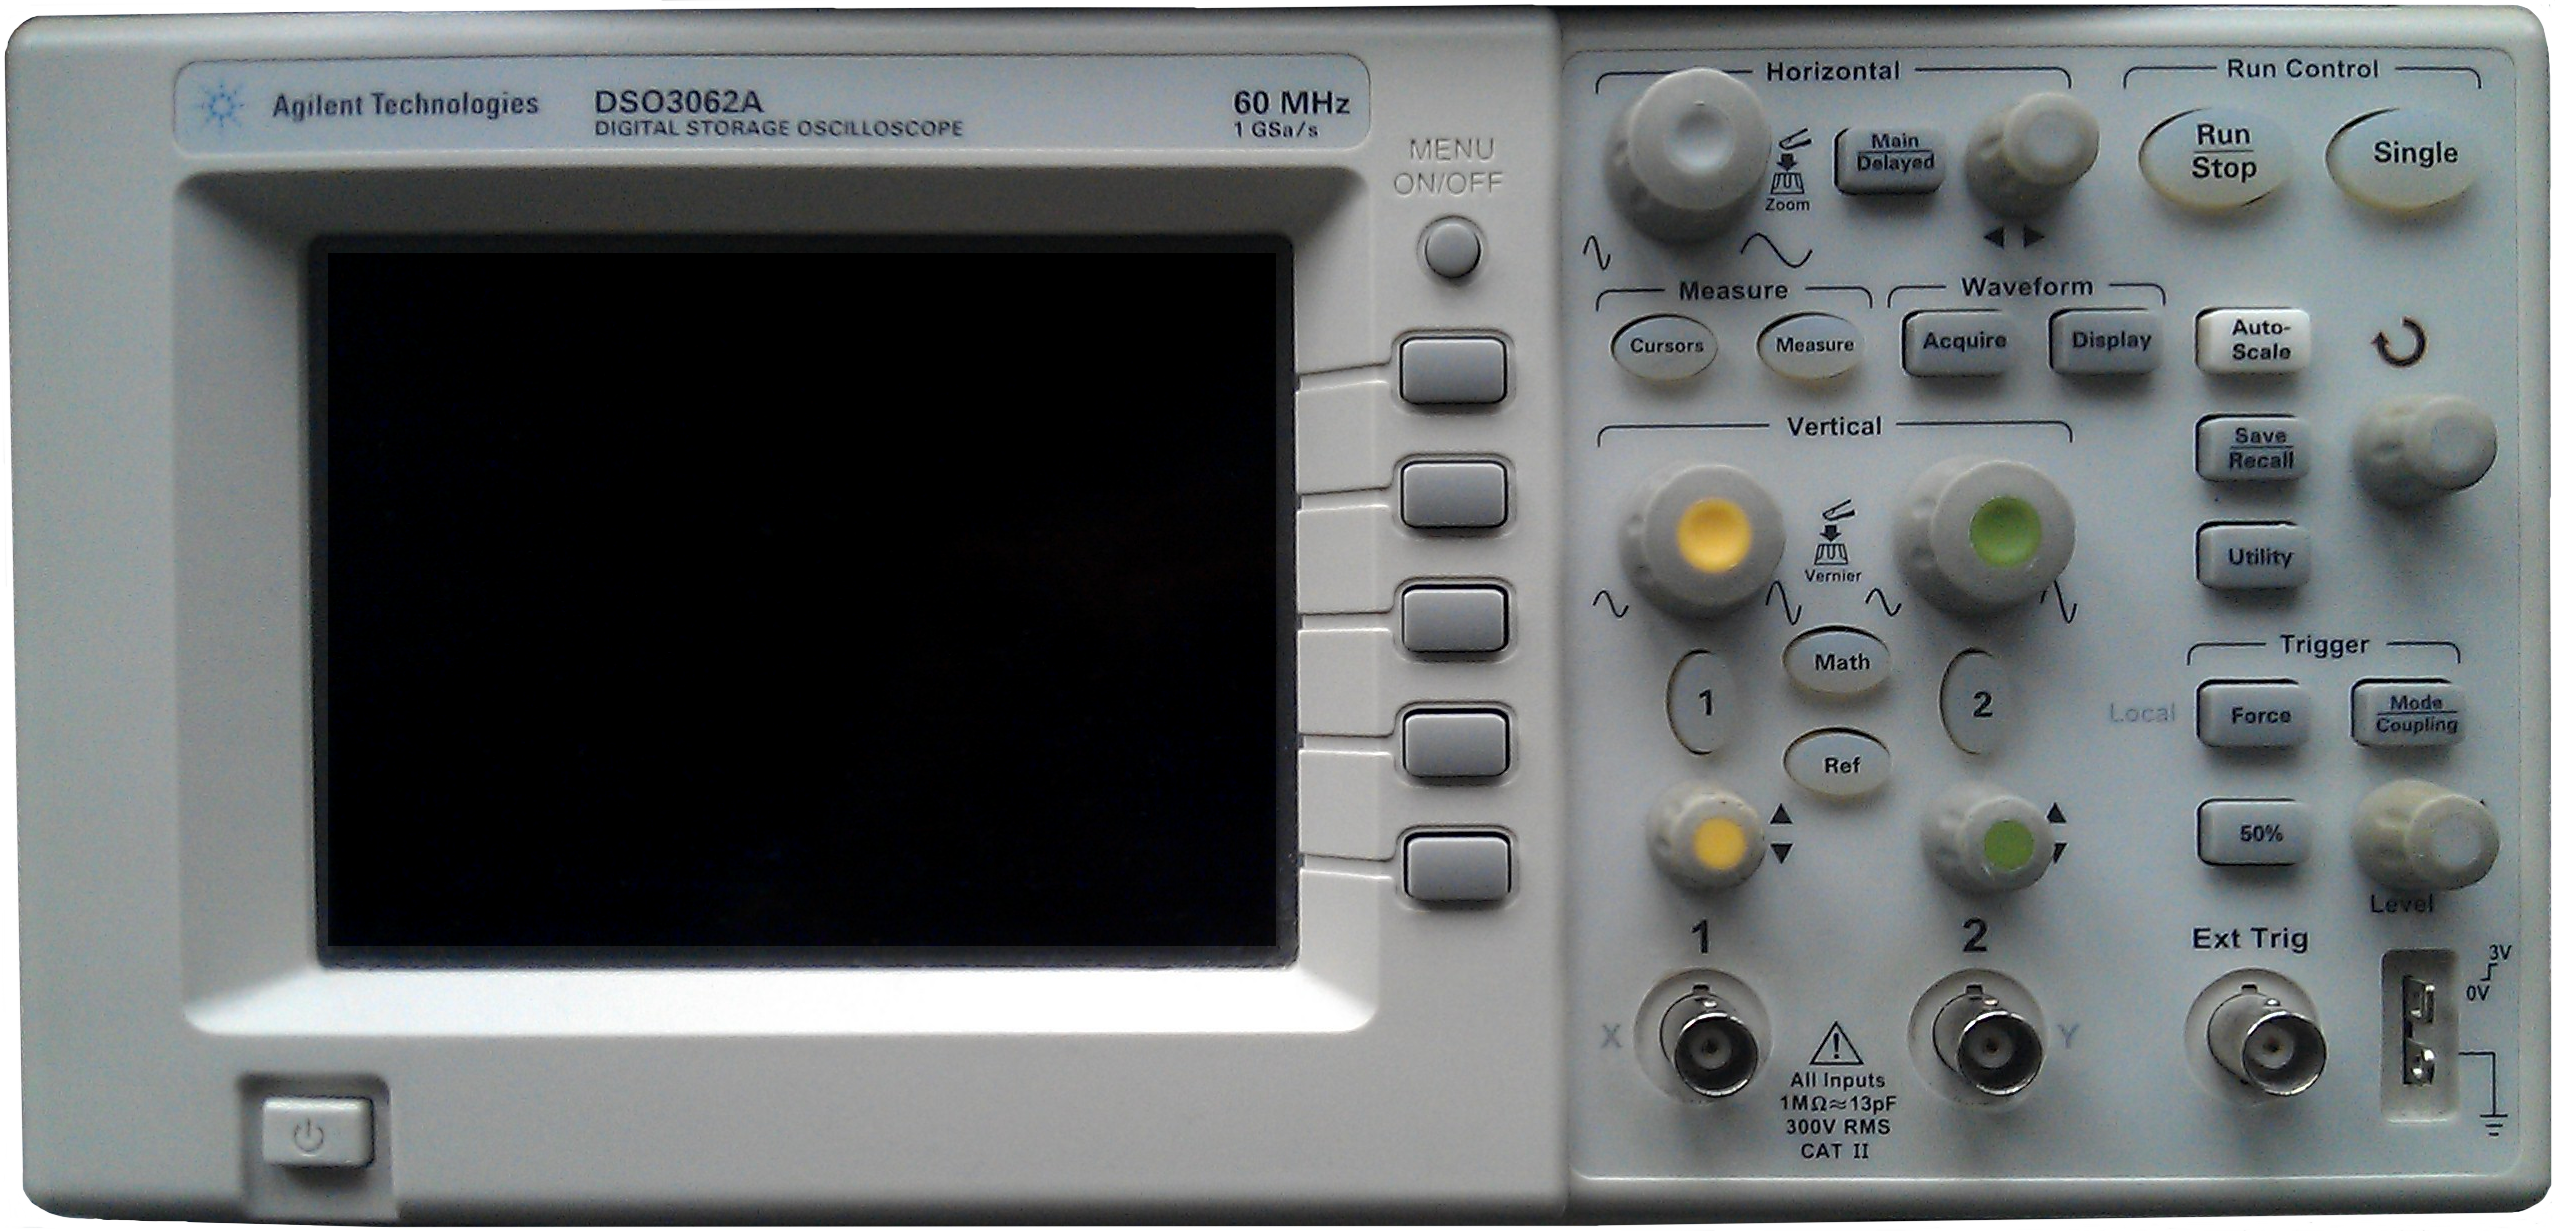
\includegraphics[scale=0.08]{Messtechnik/Bilder/oszi_foto.png}
% \vspace{-6cm}
%\end{wrapfigure}

\section*{Theorie- und Prüfungsfragen} 

\mucho{1}{TD612}
{Wie verhält sich die Frequenz eines Oszillators bei Temperaturanstieg, wenn die Kapazität des Schwingkreiskondensators mit dem Temperaturanstieg ebenfalls ansteigt?}%Frage
{Die Frequenz bleibt stabil.}%A
{Die Schwingungen reißen ab (Aussetzer).}%B
{Die Frequenz erhöht sich.}%C
{Die Frequenz verringert sich.}%D
{D}%Lösung

\mucho{2}{TD420}
{Welche Merkmale hat ein HF-Leistungsverstärker im A-Betrieb?}%Frage
{Wirkungsgrad $80$ bis $87 \%$, hoher Oberwellenanteil, der Ruhestrom ist fast null.}%A
{Wirkungsgrad bis zu $70 \%$, geringer Oberwellenanteil, geringer bis mittlerer Ruhestrom.}%B
{Wirkungsgrad bis zu $80 \%$, geringer Oberwellenanteil, sehr geringer Ruhestrom.}%C
{Wirkungsgrad ca. $40 \%$, geringst möglicher Oberwellenanteil, hoher Ruhestrom.}%D
{D}%Lösung

\mucho{3}{TD421}
{Welche Merkmale hat ein HF-Leistungsverstärker im B-Betrieb?}%Frage
{Wirkungsgrad ca. $40 \%$, geringst möglicher Oberwellenanteil, hoher Ruhestrom.}%A
{Wirkungsgrad bis zu $70 \%$, geringer Oberwellenanteil, geringer bis mittlerer Ruhestrom.}%B
{Wirkungsgrad bis zu $80 \%$, geringer Oberwellenanteil, sehr geringer Ruhestrom.
}%C
{Wirkungsgrad $80$ bis $87 \%$, hoher Oberwellenanteil, der Ruhestrom ist fast null.
}%D
{C}%Lösung


\mucho{4}{TD422}
{ Welche Merkmale hat ein HF-Leistungsverstärker im C-Betrieb?}%Frage
{Wirkungsgrad bis zu $70 \%$, geringer Oberwellenanteil, geringer bis mittlerer Ruhestrom.}%A
{Wirkungsgrad $80$ bis $87 \%$, hoher Oberwellenanteil, der Ruhestrom ist fast null.}%B
{Wirkungsgrad bis zu $80 \%$, geringer Oberwellenanteil, sehr geringer Ruhestrom.}%C
{Wirkungsgrad ca. $40 \%$, geringst möglicher Oberwellenanteil, hoher Ruhestrom.}%D
{B}%Lösung


\mucho{5}{TB904}
{Die äquivalente (effektive) Strahlungsleistung (ERP) ist}%Frage
{das Produkt aus der Leistung, die unmittelbar der Antenne zugeführt wird und ihrem Gewinnfaktor in einer Richtung, bezogen auf den Halbwellendipol.}%A
{das Produkt aus der Leistung, die unmittelbar der Antenne zugeführt wird und ihrem Gewinnfaktor in einer Richtung, bezogen auf den isotropen Kugelstrahler.}%B
{die durchschnittliche Leistung, die ein Sender unter normalen Betriebsbedingungen während einer Periode der Hochfrequenzschwingung bei der höchsten Spitze der Modulationshüllkurve der Antennenspeiseleitung zuführt.}%C
{die durchschnittliche Leistung, die ein Sender unter normalen Betriebsbedingungen an die Antennenspeiseleitung während eines Zeitintervalls abgibt, das im Verhältnis zur Periode der tiefsten Modulationsfrequenz ausreichend lang ist.}%D
{A}%Lösung

\mucho{6}{TB905}
{Die äquivalente isotrope Strahlungsleistung (EIRP) ist}%Frage
{das Produkt aus der Leistung, die unmittelbar der Antenne zugeführt wird und ihrem Gewinnfaktor in einer Richtung, bezogen auf den isotropen Kugelstrahler.}%A
{das Produkt aus der Leistung, die unmittelbar der Antenne zugeführt wird und ihrem Gewinnfaktor in einer Richtung, bezogen auf den Halbwellendipol.}%B
{die durchschnittliche Leistung, die ein Sender unter normalen Betriebsbedingungen während einer Periode der Hochfrequenzschwingung bei der höchsten Spitze der Modulationshüllkurve der Antennenspeiseleitung zuführt.}%C
{die durchschnittliche Leistung, die ein Sender unter normalen Betriebsbedingungen an die Antennenspeiseleitung während eines Zeitintervalls abgibt, das im Verhältnis zur Periode der tiefsten Modulationsfrequenz ausreichend lang ist.}%D
{A}%Lösung



\mucho{7}{TD603}
{Bei dieser Schaltung handelt es sich um\\
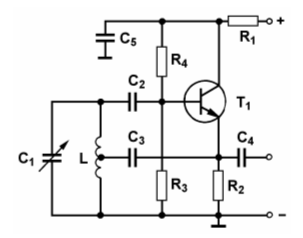
\includegraphics[scale=0.5]{Oszillator/Bilder/TD603.png}}%Frage
{einen LC-Oszillator in induktiver Dreipunktschaltung.}%A
{einen LC-Oszillator in kapazitiver Dreipunktschaltung.}%B
{einen Oberton-Oszillator in Kollektorschaltung.}%C
{einen Oberton-Oszillator in Emitterschaltung.}%D
{A}%Lösung


\mucho{8}{TD605}
{Bei dieser Oszillatorschaltung handelt es sich um einen kapazitiv rückgekoppelten Quarz-Oszillator in\\
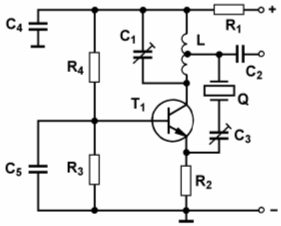
\includegraphics[scale=0.5]{Oszillator/Bilder/TD605.png}}%Frage
{Basisschaltung, in der der Quarz in Serienresonanz betrieben wird.}%A
{Basisschaltung, in der der Quarz in Parallelresonanz betrieben wird.}%B
{Emitterschaltung, in der der Quarz in Parallelresonanz betrieben wird.}%C
{Emitterschaltung, in der der Quarz in Serienresonanz betrieben wird.}%D
{A}%Lösung

\chapter{Elektromagnetisches Feld}
\begin{wrapfigure}[0]{r}[-1cm]{3cm}
 \vspace{-6cm}
 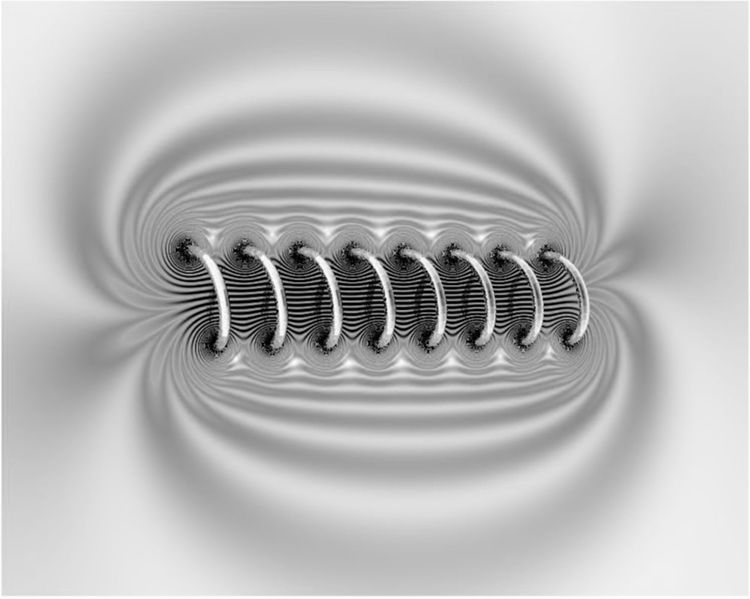
\includegraphics[scale=0.25]{elektromagnetisch/Bilder/750px-Solenoid-6.jpg}
 \vspace{-6cm}
\end{wrapfigure}

\section*{Theorie- und Prüfungsfragen} 

\mucho{1}{TB305}
{Wie nennt man das Feld zwischen zwei parallelen Kondensatorplatten bei Anschluss einer Gleichspannung?}%Frage
{Homogenes elektrisches Feld}%A
{Homogenes magnetisches Feld}%B
{Polarisiertes elektrisches Feld}%C
{Polarisiertes magnetisches Feld}%D
{A}%Lösung

\mucho{2}{TB406}
{Wenn Strom durch einen gestreckten Leiter fließt, entsteht ein}%Frage
{homogenes Magnetfeld um den Leiter.}%A
{elektrisches Feld aus konzentrischen Kreisen um den Leiter.}%B
{Magnetfeld aus konzentrischen Kreisen um den Leiter.}%C
{homogenes elektrisches Feld um den Leiter.}%D
{C}%Lösung

\mucho{3}{TB405}
{Wie nennt man das Feld im Innern einer langen Zylinderspule beim Fließen eines Gleichstroms?}
{Homogenes magnetisches Feld}%A
{Homogenes elektrisches Feld}%B
{Konzentrisches magnetisches Feld}%C
{Zentriertes magnetisches Feld}%D
{A}%Lösung


\mucho{4}{TB502}
{Wie erfolgt die Ausbreitung einer elektromagnetischen Welle? (Im folgenden Text ist H-Feld die magnetische Feldkomponente und E-Feld die elektrische Feldkomponente.)}%Frage
{Sie erfolgt durch eine sich ausbreitende Wechselwirkung zwischen E-Feld und H-Feld.}%A
{Die Ausbreitung erfolgt nur über das E-Feld. Das H-Feld ist nur im Nahfeld vorhanden.}%B
{Die Ausbreitung erfolgt nur über das H-Feld. Das E-Feld ist nur im Nahfeld vorhanden.}%C
{E-Feld und H-Feld breiten sich unabhängig voneinander aus und stehen senkrecht zueinander und zur Ausbreitungsrichtung.}%D
{A}%Lösung


\mucho{5}{TB511}
{Eine Yagiantenne mit 12,15 dBi Antennen- gewinn wird mit 250 W Senderleistung direkt gespeist. Welche elektrische Ersatzfeldstärke ergibt sich bei Freiraumausbreitung in 30 m Entfernung?}%Frage
{9,2 V/m}%A
{11,8 V/m}%B
{13,1 V/m}%C
{353 V/m}%D
{B; $P_{EIRP} = P_S \cdot 10^{\frac{g_i}{10}}; E=\dfrac{\sqrt{30\Omega \cdot P_{EIRP}}}{d}$}%Lösung

\mucho{6}{TI101}
{Welche ionosphärischen Schichten bestimmen die Fernausbreitung am Tage?}%Frage
{D-, E-, F1- und F2-Schicht}%A
{E- und F-Schicht}%B
{F1- und F2-Schicht}%C
{E- und D-Schicht}%D
{A}%Lösung

\mucho{7}{TI237}
{ Warum sind Signale im 160-, 80- und 40-Meter-Band tagsüber nur schwach und nicht für den weltweiten Funkverkehr geeignet?}%Frage
{Wegen der Tagesdämpfung in der D-Schicht.}%A
{Wegen der Tagesdämpfung in der F1-Schicht.}%B
{Wegen der Tagesdämpfung in der F2-Schicht.}%C
{Wegen der Tagesdämpfung in der A-Schicht.}%D
{A}%Lösung

\mucho{8}{TI237}
{Was bedeutet der Begriff ``Sporadic E''? Es ist}%Frage
{eine Reflexion an lokal begrenzten Bereichen mit ungewöhnlich hoher Ionisation innerhalb der E-Schicht.}%A
{eine kurzfristige, plötzliche Inversionsänderung in der E-Schicht, die Fernausbreitung im VHF-Bereich ermöglicht.}%B
{eine kurzzeitig auftretende, starke Reflexion von VHF-Signalen an Meteorbahnen innerhalb der E-Schicht.}%C
{ein lokal begrenzter, kurzzeitiger Ausfall der Reflexion durch ungewöhnlich hohe Ionisation innerhalb der E-Schicht.}%D
{A}%Lösung

\mucho{9}{TI224}
{Die MUF für eine Funkstrecke ist}%Frage
{der Mittelwert aus der höchsten und niedrigsten brauchbaren Frequenz, bei der sich elektromagnetische Wellen zwischen zwei Orten durch ionosphärische Brechung ausbreiten können.}%A
{die niedrigste brauchbaren Frequenz, bei der sich elektromagnetische Wellen zwischen zwei Orten durch ionosphärische Brechung ausbreiten können.}%B
{die vorgeschriebene nutzbare Frequenz bei der sich elektromagnetische Wellen zwischen zwei Orten durch ionosphärische Brechung ausbreiten können.}%C
{die höchste brauchbare Frequenz, bei der sich elektromagnetische Wellen zwischen zwei Orten durch ionosphärische Brechung ausbreiten können.}%D
{A}%Lösung

\mucho{10}{TI213}
{Was versteht man unter dem Begriff ``Mögel-Dellinger-Effekt''? Man versteht darunter}%Frage
{das Übersprechen der Modulation eines starken Senders auf andere, über die Ionosphäre übertragene HF-Signale.}%A
{den zeitlich begrenzten Schwund durch Mehrwegeausbreitung in der Ionosphäre.}%B
{die zeitlich begrenzt auftretende Verzerrung der Modulation.}%C
{den totalen, zeitlich begrenzten Ausfall der Reflexion an der Ionosphäre.}%D
{D}%Lösung


\chapter{Antennen}
\begin{wrapfigure}[1]{r}[0cm]{4cm}
 \vspace{-6cm}
  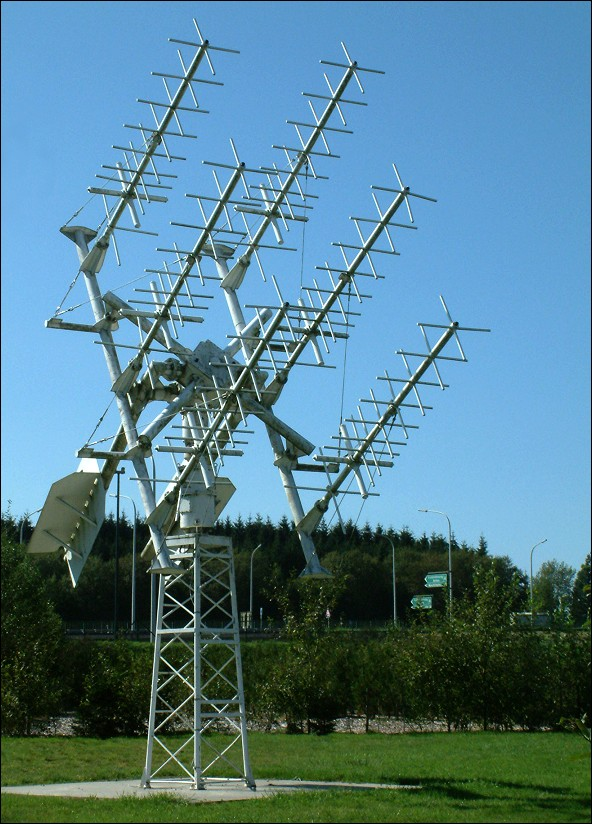
\includegraphics[scale=0.2]{Antennen/Bilder/Kreuzdipolarp.jpg}
 \vspace{-6cm}
\end{wrapfigure}

\section*{Theorie- und Prüfungsfragen}

\subsection*{Dipol}

\begin{enumerate} 
	\item \emph{\textbf{TH206}}  Ein Halbwellendipol wird auf der Grundfrequenz in der Mitte...
	\begin{enumerate}
	\itemsep1pt\parskip0pt\parsep0pt
		\item[A] spannungsgespeist.
		\item[B] stromgespeist.
		\item[C] endgespeist.
		\item[D] parallel gespeist.
		\loesung{Lösung B}
	\end{enumerate} 
	\item \emph{\textbf{TH204}}  Die Impedanz in der Mitte eines Halbwellendipols beträgt je nach Aufbauhöhe ungefähr ...
	\begin{enumerate}
	\itemsep1pt\parskip0pt\parsep0pt
		\item[A] 60 bis 120 Ohm.
		\item[B] 120 bis 240 Ohm.
		\item[C]  40 bis 80 Ohm.
		\item[D]  240 bis 600 Ohm.
		\loesung{Lösung C}
	\end{enumerate}
\end{enumerate}

\subsection*{EIRP und ERP}

\begin{enumerate} 
	\item[3] Was bedeutet der Ausdruck ERP.
		\loesung{ERP kommt von effective radio power und bedeutet ``Effektive Strahlungsleistung''}
	\item[4] Wie lässt sich die $P_{ERP}$ und $P_{EIRP}$ berechnen?
		\loesung{$P_{ERP} = (P_{Sender}-P_{Verlust}) \cdot G_{Antenne}; P_{EIRP}=1,64\cdot P_{ERP} $}
	\item[5] \emph{\textbf{TL204}}  Ein Sender mit 0,6 Watt Ausgangsleistung ist über eine Antennenleitung, die 1 dB Kabelverluste hat, an eine Richtantenne mit 11 dB Gewinn (auf Dipol bezogen) angeschlossen. Welche EIRP wird von der Antenne maximal abgestrahlt?
	\begin{enumerate}
	\itemsep1pt\parskip0pt\parsep0pt
		\item[A] $6,0W$
		\item[B] $7,8W$
		\item[C] $9,8W$
		\item[D] $12,7W$
		\loesung{Lösung C}
	\end{enumerate}
	\item[6] \emph{\textbf{TL205}}  Ein Sender mit 5 Watt Ausgangsleistung ist über eine Antennenleitung, die 2 dB Kabelverluste hat, an eine Antenne mit 5 dB Gewinn (auf Dipol bezogen) angeschlossen. Welche EIRP wird von der Antenne maximal abgestrahlt?
	\begin{enumerate}
	\itemsep1pt\parskip0pt\parsep0pt
		\item[A] $6,1W$
		\item[B] $10,0W$
		\item[C] $16,4W$
		\item[D] $32,8W$
		\loesung{Lösung C}
	\end{enumerate}
\end{enumerate}


\subsection*{Bauformen}

\begin{enumerate} 
\itemsep1pt\parskip0pt\parsep0pt
\item[1] Ordne der Abbildungen mit Schleifenantennen \ref{schleifen} folgende Bauformen zu: Dreiecksschleife (Delta Loop), Faltdipol, Quadratische Schleife (Quad Loop)
\loesung{
    Bild A zeigt einen Faltdipol.
    Bild B zeigt eine  Quadratische Schleife (Quad Loop).
    Bild C zeigt eine Dreiecksschleife (Delta Loop).
}
\end{enumerate}

\begin{figure}[H]
	\centering
	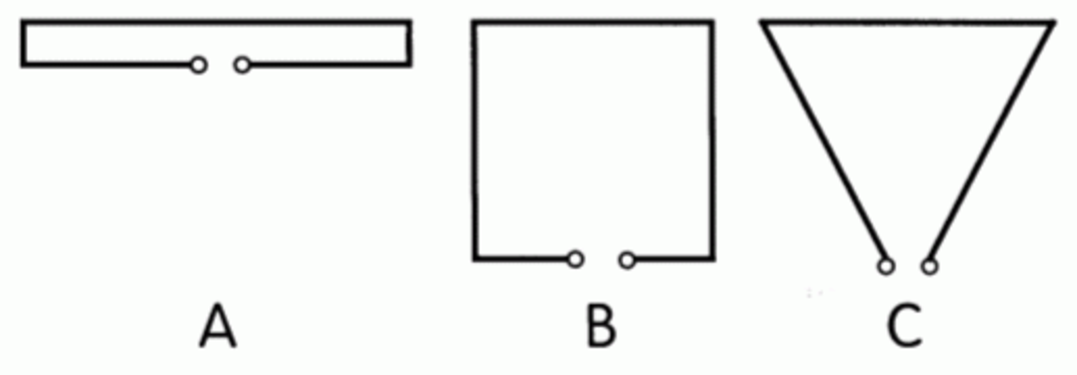
\includegraphics[scale=0.4]{Antennen/Bilder/Schleifen.pdf}
	\caption{Bauformen von Schleifenantennen}
	\label{schleifen}
\end{figure}

%------------------------------------------------------

\begin{enumerate} 
\itemsep1pt\parskip0pt\parsep0pt
\item[1] Ordne der Abbildungen mit UKW-Vertikalantennen \ref{ukw} folgende Bauformen zu: Groundplane-Antenne, Sperrtopf-Antenne, Viertelwellenstab, $\lambda/2$-Antenne, $5/8- \lambda$-Antenne
\loesung{
    Bild A zeigt einen Viertelwellenstab.
    Bild B zeigt eine  $\lambda/2$-Antenne.
    Bild C zeigt eine $5/8- \lambda$-Antenne.
    Bild D zeigt eine Sperrtopf-Antenne.
    Bild E zeigt eine Groundplane-Antenne.
}
\end{enumerate}

\begin{figure}[H]
	\centering
	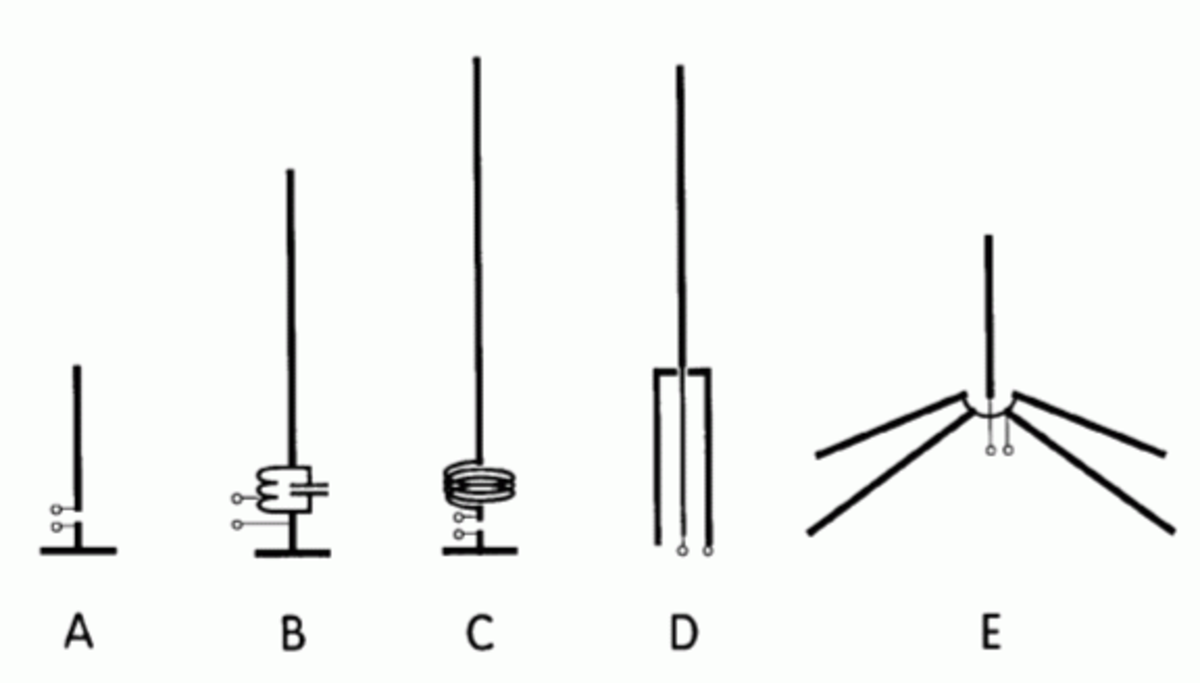
\includegraphics[scale=0.4]{Antennen/Bilder/ukw.pdf}
	\caption{Bauformen von UKW-Vertikalantennen}
	\label{ukw}
\end{figure}

%------------------------------------------------------

\begin{enumerate} 
\itemsep1pt\parskip0pt\parsep0pt
\item[1] Ordne der Abbildungen \ref{yagi} folgende Bauformen zu: horizontal polarisierte Yagi-Antenne, zirkular polarisierte X-Yagi-Antenne, Kreuz-Yagi-Antenne, vertikal polarisierte Yagi-Antenne.
\loesung{
    Bild A zeigt eine horizontal polarisierte Yagi-Antenne.
    Bild B zeigt eine vertikal polarisierte Yagi-Antenne.
    Bild C zeigt eine Kreuz-Yagi-Antenne.
    Bild D zeigt eine zirkular polarisierte X-Yagi-Antenne.
}
\end{enumerate}

\begin{figure}[H]
	\centering
	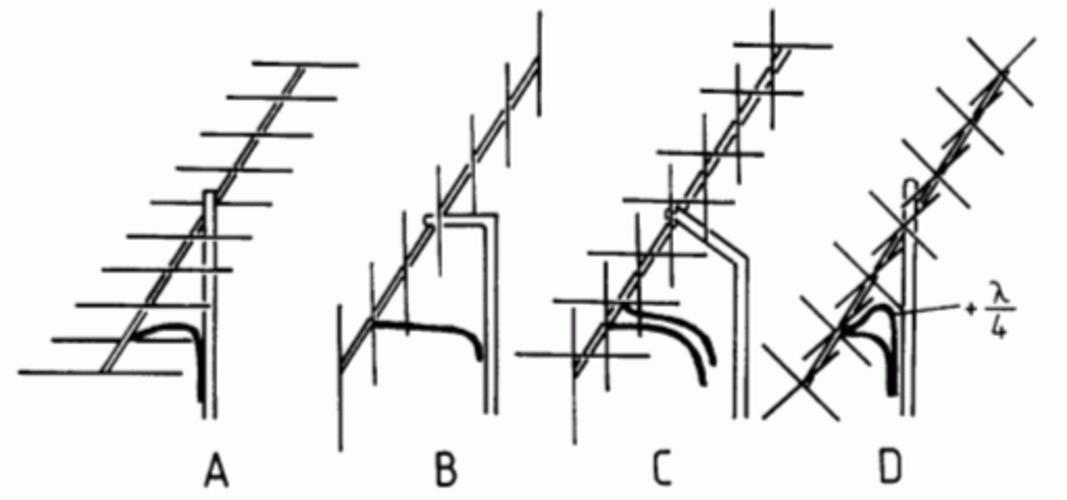
\includegraphics[scale=0.5]{Antennen/Bilder/TH209.pdf}
	\caption{Bauformen von Yagi-Antennen}
	\label{yagi}
\end{figure}
%------------------------------------------------------
\begin{enumerate} 
\itemsep1pt\parskip0pt\parsep0pt
\item[1] Ordne den Abbildungen \ref{strahlungsdiagramm} folgende Strahlungsdiagramme zu: Groundplane, Yagi-Antenne, Dipol, gibt es nicht.
\loesung{
    Bild A Dipol
    Bild B Yagi-Antenne
    Bild C Groundplane
    Bild D gibt es nicht
}
\end{enumerate}

\begin{figure}[H]
	\centering
	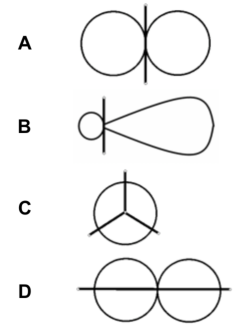
\includegraphics[scale=0.8]{Antennen/Bilder/Strahlungsdiagramm.pdf}
	\caption{Strahlungsdiagramme von Antennen}
	\label{strahlungsdiagramm}
\end{figure}


\chapter{Kabel und Leitungen}
\begin{wrapfigure}[0]{r}[0cm]{4cm}
 \vspace{-6cm}
  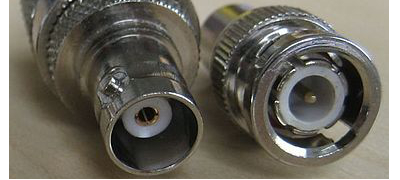
\includegraphics[scale=0.4]{KabelLeitungen/Bilder/bnc.jpg}
 \vspace{-6cm}
\end{wrapfigure}

\section*{Theorie- und Prüfungsfragen}

%--------------------------------------------


\mucho{1}{TH303}
{Im Amateurfunk übliche Koaxialkabel weisen typischerweise Wellenwiderstände von}%Frage
{50, 60 und 75 $\Omega$ auf.}%A
{50, 300 und 600 $\Omega$ auf.}%B
{60, 120 und 240 $\Omega$ auf.}%C
{50, 75 und 240 $\Omega$ auf.}%D
{A}%Lösung

\mucho{2}{TH316}
{Eine offene Paralleldrahtleitung ist aus Draht mit einem Durchmesser von 2 mm gefertigt. Der Abstand der Leiter beträgt 20 cm. Wie hoch ist der Wellenwiderstand der Leitung?}%Frage
{ca. 276 $\Omega$}%A
{ca. 635 $\Omega$}%B
{ca. 820 $\Omega$}%C
{ca. 2,8k $\Omega$}%D
{B; $Z_W = \dfrac{120\Omega}{1} \cdot ln \left( \dfrac{2\cdot 200mm}{2mm} \right) = 635,7\Omega$; für Luft $e_r=1$}%Lösung

\mucho{3}{TH313}
{Wann ist eine Speiseleitung asymmetrisch?}%Frage
{Wenn die beiden Leiter unterschiedlich geformt sind, z.B. Koaxialkabel.}%A
{Wenn die hin- und zurücklaufende Leistung verschieden sind.}%B
{Wenn sie außerhalb ihrer Resonanzfrequenz betrieben wird.}%C
{Wenn die Koaxial-Leitung Spannung gegen Erde führt.}%D
{A}%Lösung

\mucho{4}{TH314}
{Bei einer Leitung mit symmetrischer Übertragung}%Frage
{sind die Impedanzen bei beiden Leitern gegen Erde unendlich hoch.}%A
{liegt einer der beiden Leiter auf Erdpotential.}%B
{ist Strom und Spannung in den beiden Leitern gegenüber Erde gleich groß und gegenphasig.}%C
{ist Strom und Spannung in den beiden Leitern gegenüber Erde gleich groß und gleichphasig.}%D
{C}%Lösung

\mucho{5}{TH324}
{Welche Leitungen sollten für die HF-Verbindungen zwischen Einrichtungen in der Amateurfunkstelle verwendet werden, um unerwünschte Abstrahlungen zu vermeiden?}%Frage
{Unabgestimmte Speiseleitungen}%A
{Symmetrische Feederleitungen}%B
{Hochwertige asymmetrische Koaxialkabel}%C
{Hochwertige abgeschirmte Netzanschlusskabel}%D
{C}%Lösung

\mucho{6}{TH320}
{Der Verkürzungsfaktor eines Koaxialkabels mit einem Dielektrikum aus massivem Polyäthylen beträgt ungefähr}%Frage
{0,66.}%A
{0,1.}%B
{0,8.}%C
{1,0.}%D
{A; $k=\dfrac{1}{\sqrt{\epsilon_r}} = \dfrac{1}{\sqrt{2,29}} = \dfrac{1}{1,513} = 0,66  $}%Lösung

\mucho{7}{TH319}
{Der Verkürzungsfaktor einer luftisolierten Paralleldrahtleitung ist}%Frage
{0,1.}%A
{ungefähr 1}%B
{0,66.}%C
{unbestimmt}%D
{B}%Lösung

\mucho{8}{TH322}
{Welche mechanische Länge hat ein $\lambda/4$ langes Koaxkabel mit Vollpolyethylenisolierung bei 145 MHz?}%Frage
{17 cm}%A
{34,2 cm}%B
{51,7 cm}%C
{1,03 m}%D
{B; $ 
\lambda = \dfrac{300m}{f} = \dfrac{300}{145} = 2,069m; 
l_{Luft} = \dfrac{ \lambda }{4}=0,517m; 
l= 0,66 \cdot 0,517m = 34,12 cm $}%Lösung

\mucho{9}{TH306}
{Welche Dämpfung ergibt sich auf der Grundlage des Kabeldämpfungsdiagramms für ein 25-m-langes Koaxialkabel vom Typ RG213 (MIL) bei 3,5 MHz?}%Frage
{0,1 dB}%A
{1,2 dB}%B
{0,6 dB}%C
{0,3 dB}%D
{D}%Lösung

\mucho{10}{TH307}
{Welche Dämpfung ergibt sich auf der Grundlage des Kabeldämpfungsdiagramms für ein 25-m-langes Koaxialkabel vom Typ RG213U-S100 bei 29 MHz?}%Frage
{0,5 dB}%A
{2,1 dB}%B
{1,1 dB}%C
{0,2 dB}%D
{A}%Lösung

\mucho{11}{TH311}
{Welches der folgenden Kabel weist im Kurzwellenbereich den geringsten Verlust auf?}%Frage
{Kunststoffisolierte Zweidrahtleitung}%A
{Koaxialkabel mit Vollisolation}%B
{UKW-Bandleitung}%C
{Offene Zweidrahtleitung}%D
{D}%Lösung

% Literaturverzeichnis
\bibliographystyle{natdin}
\addcontentsline{toc}{section}{Literaturverzeichnis}
\bibliography{Literaturverzeichnis}
% Abbildungsverzeichnis
\newpage
\addcontentsline{toc}{section}{Abbildungsverzeichnis}
\listoffigures	
%Anhang

\end{document}


